\documentclass[twoside]{book}

% Packages required by doxygen
\usepackage{fixltx2e}
\usepackage{calc}
\usepackage{doxygen}
\usepackage[export]{adjustbox} % also loads graphicx
\usepackage{graphicx}
\usepackage[utf8]{inputenc}
\usepackage{makeidx}
\usepackage{multicol}
\usepackage{multirow}
\PassOptionsToPackage{warn}{textcomp}
\usepackage{textcomp}
\usepackage[nointegrals]{wasysym}
\usepackage[table]{xcolor}

% Font selection
\usepackage[T1]{fontenc}
\usepackage[scaled=.90]{helvet}
\usepackage{courier}
\usepackage{amssymb}
\usepackage{sectsty}
\renewcommand{\familydefault}{\sfdefault}
\allsectionsfont{%
  \fontseries{bc}\selectfont%
  \color{darkgray}%
}
\renewcommand{\DoxyLabelFont}{%
  \fontseries{bc}\selectfont%
  \color{darkgray}%
}
\newcommand{\+}{\discretionary{\mbox{\scriptsize$\hookleftarrow$}}{}{}}

% Page & text layout
\usepackage{geometry}
\geometry{%
  a4paper,%
  top=2.5cm,%
  bottom=2.5cm,%
  left=2.5cm,%
  right=2.5cm%
}
\tolerance=750
\hfuzz=15pt
\hbadness=750
\setlength{\emergencystretch}{15pt}
\setlength{\parindent}{0cm}
\setlength{\parskip}{0.2cm}
\makeatletter
\renewcommand{\paragraph}{%
  \@startsection{paragraph}{4}{0ex}{-1.0ex}{1.0ex}{%
    \normalfont\normalsize\bfseries\SS@parafont%
  }%
}
\renewcommand{\subparagraph}{%
  \@startsection{subparagraph}{5}{0ex}{-1.0ex}{1.0ex}{%
    \normalfont\normalsize\bfseries\SS@subparafont%
  }%
}
\makeatother

% Headers & footers
\usepackage{fancyhdr}
\pagestyle{fancyplain}
\fancyhead[LE]{\fancyplain{}{\bfseries\thepage}}
\fancyhead[CE]{\fancyplain{}{}}
\fancyhead[RE]{\fancyplain{}{\bfseries\leftmark}}
\fancyhead[LO]{\fancyplain{}{\bfseries\rightmark}}
\fancyhead[CO]{\fancyplain{}{}}
\fancyhead[RO]{\fancyplain{}{\bfseries\thepage}}
\fancyfoot[LE]{\fancyplain{}{}}
\fancyfoot[CE]{\fancyplain{}{}}
\fancyfoot[RE]{\fancyplain{}{\bfseries\scriptsize Generated on Fri Mar 31 2017 03\+:11\+:40 for Linda by Doxygen }}
\fancyfoot[LO]{\fancyplain{}{\bfseries\scriptsize Generated on Fri Mar 31 2017 03\+:11\+:40 for Linda by Doxygen }}
\fancyfoot[CO]{\fancyplain{}{}}
\fancyfoot[RO]{\fancyplain{}{}}
\renewcommand{\footrulewidth}{0.4pt}
\renewcommand{\chaptermark}[1]{%
  \markboth{#1}{}%
}
\renewcommand{\sectionmark}[1]{%
  \markright{\thesection\ #1}%
}

% Indices & bibliography
\usepackage{natbib}
\usepackage[titles]{tocloft}
\setcounter{tocdepth}{3}
\setcounter{secnumdepth}{5}
\makeindex

% Hyperlinks (required, but should be loaded last)
\usepackage{ifpdf}
\ifpdf
  \usepackage[pdftex,pagebackref=true]{hyperref}
\else
  \usepackage[ps2pdf,pagebackref=true]{hyperref}
\fi
\hypersetup{%
  colorlinks=true,%
  linkcolor=blue,%
  citecolor=blue,%
  unicode%
}

% Custom commands
\newcommand{\clearemptydoublepage}{%
  \newpage{\pagestyle{empty}\cleardoublepage}%
}


%===== C O N T E N T S =====

\begin{document}

% Titlepage & ToC
\hypersetup{pageanchor=false,
             bookmarks=true,
             bookmarksnumbered=true,
             pdfencoding=unicode
            }
\pagenumbering{roman}
\begin{titlepage}
\vspace*{7cm}
\begin{center}%
{\Large Linda \\[1ex]\large 0.\+1 }\\
\vspace*{1cm}
{\large Generated by Doxygen 1.8.10}\\
\vspace*{0.5cm}
{\small Fri Mar 31 2017 03:11:40}\\
\end{center}
\end{titlepage}
\clearemptydoublepage
\tableofcontents
\clearemptydoublepage
\pagenumbering{arabic}
\hypersetup{pageanchor=true}

%--- Begin generated contents ---
\chapter{Hierarchical Index}
\section{Class Hierarchy}
This inheritance list is sorted roughly, but not completely, alphabetically\+:\begin{DoxyCompactList}
\item \contentsline{section}{Linda}{\pageref{class_linda}}{}
\begin{DoxyCompactList}
\item \contentsline{section}{Linda\+Model}{\pageref{class_linda_model}}{}
\end{DoxyCompactList}
\item \contentsline{section}{Linda\+Row\+Model}{\pageref{class_linda_row_model}}{}
\end{DoxyCompactList}

\chapter{Data Structure Index}
\section{Data Structures}
Here are the data structures with brief descriptions\+:\begin{DoxyCompactList}
\item\contentsline{section}{\hyperlink{class_linda}{Linda} \\*\hyperlink{class_linda}{Linda} is a Database Abstraction Layer for P\+H\+P Built on top P\+D\+O }{\pageref{class_linda}}{}
\item\contentsline{section}{\hyperlink{class_linda_model}{Linda\+Model} \\*\hyperlink{class_linda_model}{Linda\+Model} is an Active-\/record based O\+R\+M, it facilitates the creation and use of business objects whose data requires persistent storage to a database. It is an implementation of the Active Record pattern which itself is a description of an Object Relational Mapping system }{\pageref{class_linda_model}}{}
\item\contentsline{section}{\hyperlink{class_linda_row_model}{Linda\+Row\+Model} }{\pageref{class_linda_row_model}}{}
\end{DoxyCompactList}

\chapter{File Index}
\section{File List}
Here is a list of all files with brief descriptions\+:\begin{DoxyCompactList}
\item\contentsline{section}{C\+:/\+Apache24/htdocs/easygo/process/\+Linda/\hyperlink{_linda_8inc}{Linda.\+inc} }{\pageref{_linda_8inc}}{}
\item\contentsline{section}{C\+:/\+Apache24/htdocs/easygo/process/\+Linda/\hyperlink{_linda_8php}{Linda.\+php} }{\pageref{_linda_8php}}{}
\item\contentsline{section}{C\+:/\+Apache24/htdocs/easygo/process/\+Linda/\hyperlink{_linda_model_8php}{Linda\+Model.\+php} }{\pageref{_linda_model_8php}}{}
\item\contentsline{section}{C\+:/\+Apache24/htdocs/easygo/process/\+Linda/\hyperlink{_linda_row_model_8php}{Linda\+Row\+Model.\+php} }{\pageref{_linda_row_model_8php}}{}
\end{DoxyCompactList}

\chapter{Data Structure Documentation}
\hypertarget{class_linda}{}\section{Linda Class Reference}
\label{class_linda}\index{Linda@{Linda}}


\hyperlink{class_linda}{Linda} is a Database Abstraction Layer for P\+H\+P Built on top P\+D\+O.  


Inheritance diagram for Linda\+:\begin{figure}[H]
\begin{center}
\leavevmode
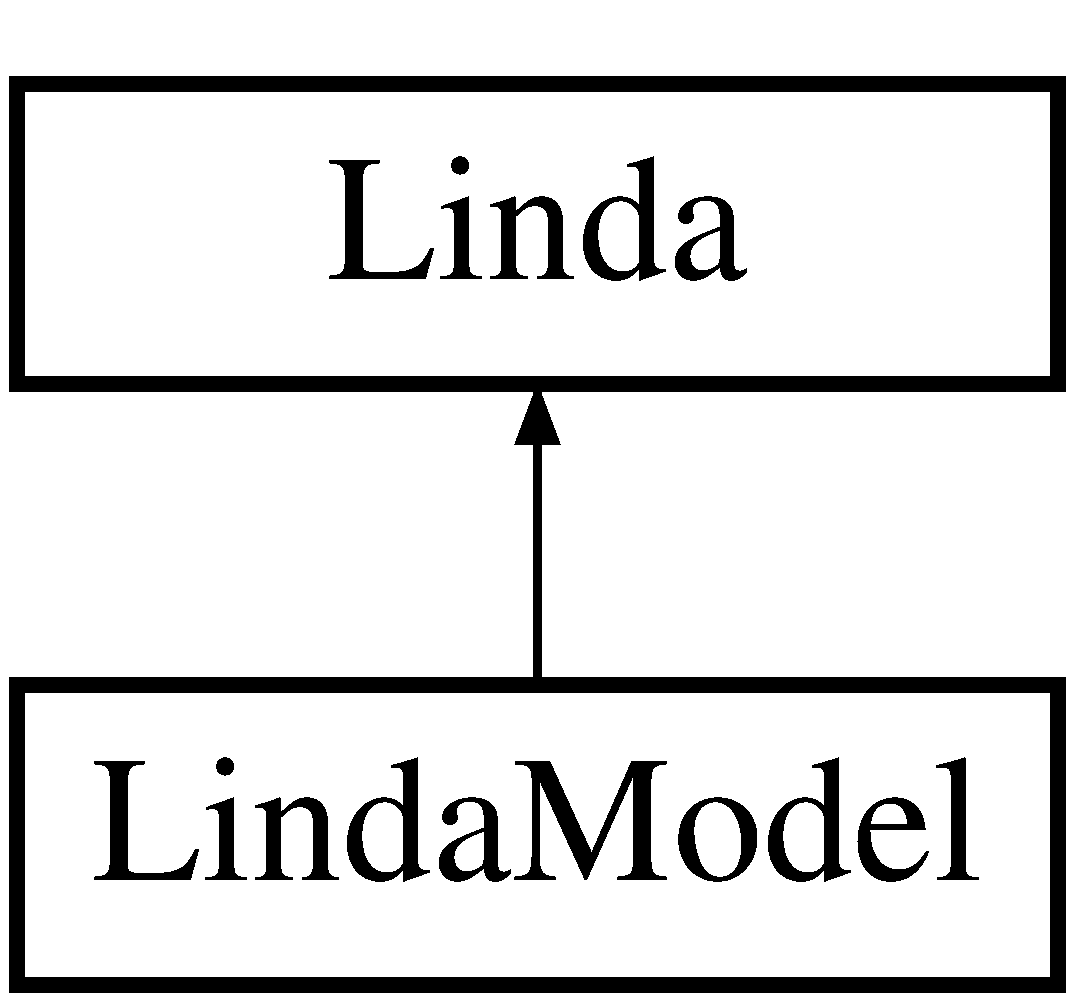
\includegraphics[height=2.000000cm]{class_linda}
\end{center}
\end{figure}
\subsection*{Public Member Functions}
\begin{DoxyCompactItemize}
\item 
\hyperlink{class_linda_a095c5d389db211932136b53f25f39685}{\+\_\+\+\_\+construct} ()
\item 
\hyperlink{class_linda_aaded27ecadbc8530b9b21cbb38dfa4a8}{set\+Table} (\$table\+Name)
\item 
\hyperlink{class_linda_a87d58413379d402e5dee4f5825b686fd}{fetch} (\$fields, \$query\+Config=array())
\item 
\hyperlink{class_linda_ac000dfba7a410bb147dc77571d1e2ed5}{update} (\$fields, \$query\+Config)
\item 
\hyperlink{class_linda_af5a8f159a27ca700aa869092a5696be1}{put} (\$fields, \$values)
\item 
\hyperlink{class_linda_a8a141e762ceb79165d9a049eaa718d38}{delete} (\$query\+Config)
\item 
\hyperlink{class_linda_ad2e4fa0b57c9acdf15cd932346381af5}{run\+Query} ()
\item 
\hyperlink{class_linda_a3292920004f4f0eb71524e2e871fd9cc}{count} (\$column\+Name, \$val, \$operator=\char`\"{}=\char`\"{})
\item 
\hyperlink{class_linda_a9405f06abe08887d915b8c0a98885cb2}{max\+\_\+in\+\_\+column} (\$column\+Name)
\item 
\hyperlink{class_linda_ace93ec905a1eba8f431c1d6bb279ac20}{max\+Row} (\$field\+Name)
\item 
\hyperlink{class_linda_a47a8d3c75c7454aca40d3b7808465ab6}{min\+\_\+in\+\_\+column} (\$column\+Name)
\item 
\hyperlink{class_linda_a94e9b7b94a61bc48ad5d866bc93670ce}{min\+Row} (\$column\+Name)
\item 
\hyperlink{class_linda_ab39eb2457d23f38ac50e0af64a55f6e9}{sum} (\$field\+Name)
\item 
\hyperlink{class_linda_aba0d5b303383fb5b1fabb5fd01cd3800}{get\+All} ()
\item 
\hyperlink{class_linda_a15fff7e5f77cd6a7e7656e3e46b20a5c}{get\+Row\+At\+Index} (\$index)
\item 
\hyperlink{class_linda_af37433a300db1f607ee789d22828a0a0}{num\+Rows} ()
\item 
\hyperlink{class_linda_af0d2b98b49496eaef856a5b277fa775b}{peek} ()
\item 
\hyperlink{class_linda_a45fd7828ad0376368f5c32b64d5dbac4}{tail} ()
\item 
\hyperlink{class_linda_a046b5f5e8b171d4724f2780303239825}{even} ()
\item 
\hyperlink{class_linda_a666c4ea82d473f0e68ad97e3f33d1e83}{odd} ()
\item 
\hyperlink{class_linda_a421831a265621325e1fdd19aace0c758}{\+\_\+\+\_\+destruct} ()
\end{DoxyCompactItemize}
\subsection*{Data Fields}
\begin{DoxyCompactItemize}
\item 
\hyperlink{class_linda_ab7d7da38a7a04e1f95bc46697f8d80e3}{\$\+L\+I\+N\+D\+A\+\_\+\+E\+R\+R\+O\+R} = N\+U\+L\+L
\item 
\hyperlink{class_linda_a5ed9b689dc54a1e48103d904af6885a5}{\$\+C\+U\+R\+R\+E\+N\+T\+\_\+\+Q\+U\+E\+R\+Y}
\item 
const \hyperlink{class_linda_a4771733014ade9011a85f4d01b24f2fe}{Linda\+\_\+\+D\+B\+\_\+\+H\+O\+S\+T} = \hyperlink{_linda_8inc_a86b40c589d474db371ea58296a5eeb12}{L\+I\+N\+D\+A\+\_\+\+D\+B\+\_\+\+H\+O\+S\+T}
\item 
const \hyperlink{class_linda_aab80e54270eaebb370e54ec5232be43a}{Linda\+\_\+\+D\+B\+\_\+\+N\+A\+M\+E} = \hyperlink{_linda_8inc_a4e480c562d1f6701e89f603607ddbb54}{L\+I\+N\+D\+A\+\_\+\+D\+B\+\_\+\+N\+A\+M\+E}
\item 
const \hyperlink{class_linda_af392abe38a40b56515eb835fa3c39d8c}{Linda\+\_\+\+D\+B\+\_\+\+T\+Y\+P\+E} = \hyperlink{_linda_8inc_a75c0048bcb27b8bf9d4e9fd1b9eb023b}{L\+I\+N\+D\+A\+\_\+\+D\+B\+\_\+\+T\+Y\+P\+E}
\item 
const \hyperlink{class_linda_a73fe432dd03d1c21aa74940da5c04dc0}{Linda\+\_\+\+D\+B\+\_\+\+U\+S\+E\+R} = \hyperlink{_linda_8inc_a713707c7fea371f7f3892136c1e852f0}{L\+I\+N\+D\+A\+\_\+\+D\+B\+\_\+\+U\+S\+E\+R}
\item 
const \hyperlink{class_linda_a392451b719cb6bb9b0c372832ad9e6d8}{Linda\+\_\+\+D\+B\+\_\+\+P\+A\+S\+S\+W} = \hyperlink{_linda_8inc_aef9b254dff90502b875151a93b462df1}{L\+I\+N\+D\+A\+\_\+\+D\+B\+\_\+\+P\+A\+S\+S\+W}
\end{DoxyCompactItemize}
\subsection*{Protected Member Functions}
\begin{DoxyCompactItemize}
\item 
\hyperlink{class_linda_a3749f401c64588bfbecbcc3b2c1a24e4}{parse\+Model} ()
\item 
\hyperlink{class_linda_a0cee7c433eda5db6e7610d4e0dcedf99}{sanitize} (\$inp)
\item 
\hyperlink{class_linda_a190c686da9f77d10964e06f0480c9b44}{create\+Insert} (\$fields, \$inserts)
\item 
\hyperlink{class_linda_a9aa9a275e880b4446ec390cc2ba351cd}{string\+\_\+or\+\_\+int} (\$val)
\item 
\hyperlink{class_linda_aeb66ebf99ca730ea67c612735a6576b4}{query\+Builder} (\$mode, \$fields, \$query\+Config)
\end{DoxyCompactItemize}
\subsection*{Protected Attributes}
\begin{DoxyCompactItemize}
\item 
\hyperlink{class_linda_a11c2781ac527a1c951d9035f2d0197cc}{\$\+D\+B\+\_\+\+L\+I\+N\+K}
\item 
\hyperlink{class_linda_a486c281995ea6cdb9fb0367b6e260b76}{\$\+T\+A\+B\+L\+E\+\_\+\+M\+O\+D\+E\+L}
\item 
\hyperlink{class_linda_a46c628c6bd56ec5880da2515cf352183}{\$\+M\+O\+D\+E\+L\+\_\+\+S\+C\+H\+E\+M\+A} = array()
\item 
\hyperlink{class_linda_a97365f1875db5efbdefc5faa71249ff1}{\$\+D\+E\+F\+A\+U\+L\+T\+\_\+\+L\+I\+M\+I\+T} = 1000
\item 
\hyperlink{class_linda_a803cce07cc3e3f9937b6e5faba4100fe}{\$\+D\+E\+F\+A\+U\+L\+T\+\_\+\+S\+T\+A\+R\+T\+\_\+\+I\+N\+D\+E\+X} = 0
\item 
\hyperlink{class_linda_a64270a514fbca17fe7347df6320fc4ba}{\$result\+Object} = N\+U\+L\+L
\item 
\hyperlink{class_linda_a038edab690e03aff9c70a1f63c06f27e}{\$last\+Affected\+Row\+Count} = 0
\item 
\hyperlink{class_linda_aea7d038e46660f55592569906cf09494}{\$query\+Config} = array()
\end{DoxyCompactItemize}


\subsection{Detailed Description}
\hyperlink{class_linda}{Linda} is a Database Abstraction Layer for P\+H\+P Built on top P\+D\+O. 

\begin{DoxyAuthor}{Author}
Olubodun Agbalaya. 
\end{DoxyAuthor}
\begin{Desc}
\item[Examples\+: ]\par
\hyperlink{_c_1_2_apache24_2htdocs_2easygo_2process_2_linda_2_linda_8php-example}{C\+:/\+Apache24/htdocs/easygo/process/\+Linda/\+Linda.\+php}.\end{Desc}


Definition at line 11 of file Linda.\+php.



\subsection{Constructor \& Destructor Documentation}
\hypertarget{class_linda_a095c5d389db211932136b53f25f39685}{}\index{Linda@{Linda}!\+\_\+\+\_\+construct@{\+\_\+\+\_\+construct}}
\index{\+\_\+\+\_\+construct@{\+\_\+\+\_\+construct}!Linda@{Linda}}
\subsubsection[{\+\_\+\+\_\+construct()}]{\setlength{\rightskip}{0pt plus 5cm}\+\_\+\+\_\+construct (
\begin{DoxyParamCaption}
{}
\end{DoxyParamCaption}
)}\label{class_linda_a095c5d389db211932136b53f25f39685}
\begin{Desc}
\item[Examples\+: ]\par
\hyperlink{_c_1_2_apache24_2htdocs_2easygo_2process_2_linda_2_linda_8php-example}{C\+:/\+Apache24/htdocs/easygo/process/\+Linda/\+Linda.\+php}.\end{Desc}


Definition at line 30 of file Linda.\+php.

\hypertarget{class_linda_a421831a265621325e1fdd19aace0c758}{}\index{Linda@{Linda}!\+\_\+\+\_\+destruct@{\+\_\+\+\_\+destruct}}
\index{\+\_\+\+\_\+destruct@{\+\_\+\+\_\+destruct}!Linda@{Linda}}
\subsubsection[{\+\_\+\+\_\+destruct()}]{\setlength{\rightskip}{0pt plus 5cm}\+\_\+\+\_\+destruct (
\begin{DoxyParamCaption}
{}
\end{DoxyParamCaption}
)}\label{class_linda_a421831a265621325e1fdd19aace0c758}
\begin{Desc}
\item[Examples\+: ]\par
\hyperlink{_c_1_2_apache24_2htdocs_2easygo_2process_2_linda_2_linda_8php-example}{C\+:/\+Apache24/htdocs/easygo/process/\+Linda/\+Linda.\+php}.\end{Desc}


Definition at line 718 of file Linda.\+php.



\subsection{Member Function Documentation}
\hypertarget{class_linda_a3292920004f4f0eb71524e2e871fd9cc}{}\index{Linda@{Linda}!count@{count}}
\index{count@{count}!Linda@{Linda}}
\subsubsection[{count(\$column\+Name, \$val, \$operator=""="")}]{\setlength{\rightskip}{0pt plus 5cm}count (
\begin{DoxyParamCaption}
\item[{}]{\$column\+Name, }
\item[{}]{\$val, }
\item[{}]{\$operator = {\ttfamily \char`\"{}=\char`\"{}}}
\end{DoxyParamCaption}
)}\label{class_linda_a3292920004f4f0eb71524e2e871fd9cc}
Count the number of rows matching a value in a field, this method executes a query directly on the table and doesnt work on the retrieved/stored data -\/ so you must have set the table using the \hyperlink{class_linda_aaded27ecadbc8530b9b21cbb38dfa4a8}{set\+Table} method, prior to calling 
\begin{DoxyParams}[1]{Parameters}
string & {\em \$column\+Name} & field to count values from \\
\hline
string & {\em \$val} & value to be matched \\
\hline
string & {\em \$operator} & Optional operator to be used default in matching defaults to equals (=), other candidates are ( $<$, $>$ , $<$$>$) \\
\hline
\end{DoxyParams}
\begin{DoxyReturn}{Returns}
\$this 
\end{DoxyReturn}
\begin{Desc}
\item[Examples\+: ]\par
\hyperlink{_c_1_2_apache24_2htdocs_2easygo_2process_2_linda_2_linda_8php-example}{C\+:/\+Apache24/htdocs/easygo/process/\+Linda/\+Linda.\+php}.\end{Desc}


Definition at line 547 of file Linda.\+php.

\hypertarget{class_linda_a190c686da9f77d10964e06f0480c9b44}{}\index{Linda@{Linda}!create\+Insert@{create\+Insert}}
\index{create\+Insert@{create\+Insert}!Linda@{Linda}}
\subsubsection[{create\+Insert(\$fields, \$inserts)}]{\setlength{\rightskip}{0pt plus 5cm}create\+Insert (
\begin{DoxyParamCaption}
\item[{}]{\$fields, }
\item[{}]{\$inserts}
\end{DoxyParamCaption}
)\hspace{0.3cm}{\ttfamily [protected]}}\label{class_linda_a190c686da9f77d10964e06f0480c9b44}
\begin{Desc}
\item[Examples\+: ]\par
\hyperlink{_c_1_2_apache24_2htdocs_2easygo_2process_2_linda_2_linda_8php-example}{C\+:/\+Apache24/htdocs/easygo/process/\+Linda/\+Linda.\+php}.\end{Desc}


Definition at line 234 of file Linda.\+php.

\hypertarget{class_linda_a8a141e762ceb79165d9a049eaa718d38}{}\index{Linda@{Linda}!delete@{delete}}
\index{delete@{delete}!Linda@{Linda}}
\subsubsection[{delete(\$query\+Config)}]{\setlength{\rightskip}{0pt plus 5cm}delete (
\begin{DoxyParamCaption}
\item[{}]{\$query\+Config}
\end{DoxyParamCaption}
)}\label{class_linda_a8a141e762ceb79165d9a049eaa718d38}
Deletes data from a table


\begin{DoxyParams}[1]{Parameters}
type & {\em \$query\+Config,see} & \#insert for structure of the query\+Config parameter \\
\hline
\end{DoxyParams}


Definition at line 203 of file Linda.\+php.

\hypertarget{class_linda_a046b5f5e8b171d4724f2780303239825}{}\index{Linda@{Linda}!even@{even}}
\index{even@{even}!Linda@{Linda}}
\subsubsection[{even()}]{\setlength{\rightskip}{0pt plus 5cm}even (
\begin{DoxyParamCaption}
{}
\end{DoxyParamCaption}
)}\label{class_linda_a046b5f5e8b171d4724f2780303239825}
Returns even indexes from the stored result set \begin{DoxyReturn}{Returns}
array() 
\end{DoxyReturn}
\begin{Desc}
\item[Examples\+: ]\par
\hyperlink{_c_1_2_apache24_2htdocs_2easygo_2process_2_linda_2_linda_8php-example}{C\+:/\+Apache24/htdocs/easygo/process/\+Linda/\+Linda.\+php}.\end{Desc}


Definition at line 691 of file Linda.\+php.

\hypertarget{class_linda_a87d58413379d402e5dee4f5825b686fd}{}\index{Linda@{Linda}!fetch@{fetch}}
\index{fetch@{fetch}!Linda@{Linda}}
\subsubsection[{fetch(\$fields, \$query\+Config=array())}]{\setlength{\rightskip}{0pt plus 5cm}fetch (
\begin{DoxyParamCaption}
\item[{}]{\$fields, }
\item[{}]{\$query\+Config = {\ttfamily array()}}
\end{DoxyParamCaption}
)}\label{class_linda_a87d58413379d402e5dee4f5825b686fd}
The get method fetches data from the table 
\begin{DoxyParams}{Parameters}
{\em array()} & $\vert$ string \$feilds An associative array containing fields to get from the table, or the string $\ast$ \\
\hline
{\em array()} & \$query\+Config A configuration array, that contains option for the get operation\\
\hline
\end{DoxyParams}
@ \$query\+Config = array( \begin{DoxyVerb}               "whereGroup" => array(  
                 [
                     "actor_id"=>array("value"=>5, "operator"=>"="),
                    "last_name"=>array("value"=>"'%ER", "operator"=>"LIKE"),
                    "comparisonOp"=>"AND",
                    "nextOp"=>"OR"
                  ],

               [
     "actor_id"=>array("value"=>"last_name", "operator"=>"LIKE")

               ] ),




                "where_in"=>array(
                       fieldName => "id",
                       options => " 10, 15, 22,
                         query => "",
                        operator = > "AND"

                    ),

               "innerJoinGroup" => array(
                 [
                 table => "table_name",
                 conditional_column_a => "column name" 
                 conditional_column_b => "column name" 
                 ],
                 [
               table => "table_name",
                 conditional_column => "column name" 
                 ]


               ) ,

                "limit" =>[
                         index => 2,
                         count =>18

                       ],

          )\end{DoxyVerb}
 \begin{Desc}
\item[Examples\+: ]\par
\hyperlink{_c_1_2_apache24_2htdocs_2easygo_2process_2_linda_2_linda_8php-example}{C\+:/\+Apache24/htdocs/easygo/process/\+Linda/\+Linda.\+php}.\end{Desc}


Definition at line 144 of file Linda.\+php.

\hypertarget{class_linda_aba0d5b303383fb5b1fabb5fd01cd3800}{}\index{Linda@{Linda}!get\+All@{get\+All}}
\index{get\+All@{get\+All}!Linda@{Linda}}
\subsubsection[{get\+All()}]{\setlength{\rightskip}{0pt plus 5cm}get\+All (
\begin{DoxyParamCaption}
{}
\end{DoxyParamCaption}
)}\label{class_linda_aba0d5b303383fb5b1fabb5fd01cd3800}
Returns the entire result set as an array  array() \begin{Desc}
\item[Examples\+: ]\par
\hyperlink{_c_1_2_apache24_2htdocs_2easygo_2process_2_linda_2_linda_8php-example}{C\+:/\+Apache24/htdocs/easygo/process/\+Linda/\+Linda.\+php}.\end{Desc}


Definition at line 637 of file Linda.\+php.

\hypertarget{class_linda_a15fff7e5f77cd6a7e7656e3e46b20a5c}{}\index{Linda@{Linda}!get\+Row\+At\+Index@{get\+Row\+At\+Index}}
\index{get\+Row\+At\+Index@{get\+Row\+At\+Index}!Linda@{Linda}}
\subsubsection[{get\+Row\+At\+Index(\$index)}]{\setlength{\rightskip}{0pt plus 5cm}get\+Row\+At\+Index (
\begin{DoxyParamCaption}
\item[{}]{\$index}
\end{DoxyParamCaption}
)}\label{class_linda_a15fff7e5f77cd6a7e7656e3e46b20a5c}
Returns the row at a particular index in the result set \begin{DoxyReturn}{Returns}
integer 
\end{DoxyReturn}
\begin{Desc}
\item[Examples\+: ]\par
\hyperlink{_c_1_2_apache24_2htdocs_2easygo_2process_2_linda_2_linda_8php-example}{C\+:/\+Apache24/htdocs/easygo/process/\+Linda/\+Linda.\+php}.\end{Desc}


Definition at line 652 of file Linda.\+php.

\hypertarget{class_linda_a9405f06abe08887d915b8c0a98885cb2}{}\index{Linda@{Linda}!max\+\_\+in\+\_\+column@{max\+\_\+in\+\_\+column}}
\index{max\+\_\+in\+\_\+column@{max\+\_\+in\+\_\+column}!Linda@{Linda}}
\subsubsection[{max\+\_\+in\+\_\+column(\$column\+Name)}]{\setlength{\rightskip}{0pt plus 5cm}max\+\_\+in\+\_\+column (
\begin{DoxyParamCaption}
\item[{}]{\$column\+Name}
\end{DoxyParamCaption}
)}\label{class_linda_a9405f06abe08887d915b8c0a98885cb2}
Returns the maximum value on a field, this method executes a query directly on the table and doesnt work on the retrieved/stored data -\/ so you must have set the table using the \hyperlink{class_linda_aaded27ecadbc8530b9b21cbb38dfa4a8}{set\+Table} method, prior to calling 
\begin{DoxyParams}[1]{Parameters}
string & {\em \$column\+Name} & field to get the minimum value from \\
\hline
\end{DoxyParams}
\begin{DoxyReturn}{Returns}
integer 
\end{DoxyReturn}
\begin{Desc}
\item[Examples\+: ]\par
\hyperlink{_c_1_2_apache24_2htdocs_2easygo_2process_2_linda_2_linda_8php-example}{C\+:/\+Apache24/htdocs/easygo/process/\+Linda/\+Linda.\+php}.\end{Desc}


Definition at line 563 of file Linda.\+php.

\hypertarget{class_linda_ace93ec905a1eba8f431c1d6bb279ac20}{}\index{Linda@{Linda}!max\+Row@{max\+Row}}
\index{max\+Row@{max\+Row}!Linda@{Linda}}
\subsubsection[{max\+Row(\$field\+Name)}]{\setlength{\rightskip}{0pt plus 5cm}max\+Row (
\begin{DoxyParamCaption}
\item[{}]{\$field\+Name}
\end{DoxyParamCaption}
)}\label{class_linda_ace93ec905a1eba8f431c1d6bb279ac20}
Returns row containing the maximum value of a particular column, this method executes a query directly on the table and doesnt work on the retrieved/stored data -\/ so you must have set the table using the \hyperlink{class_linda_aaded27ecadbc8530b9b21cbb38dfa4a8}{set\+Table} method, prior to calling 
\begin{DoxyParams}[1]{Parameters}
string & {\em \$column\+Name} & field to get the maximum value from \\
\hline
\end{DoxyParams}
\begin{DoxyReturn}{Returns}
array() 
\end{DoxyReturn}
\begin{Desc}
\item[Examples\+: ]\par
\hyperlink{_c_1_2_apache24_2htdocs_2easygo_2process_2_linda_2_linda_8php-example}{C\+:/\+Apache24/htdocs/easygo/process/\+Linda/\+Linda.\+php}.\end{Desc}


Definition at line 579 of file Linda.\+php.

\hypertarget{class_linda_a47a8d3c75c7454aca40d3b7808465ab6}{}\index{Linda@{Linda}!min\+\_\+in\+\_\+column@{min\+\_\+in\+\_\+column}}
\index{min\+\_\+in\+\_\+column@{min\+\_\+in\+\_\+column}!Linda@{Linda}}
\subsubsection[{min\+\_\+in\+\_\+column(\$column\+Name)}]{\setlength{\rightskip}{0pt plus 5cm}min\+\_\+in\+\_\+column (
\begin{DoxyParamCaption}
\item[{}]{\$column\+Name}
\end{DoxyParamCaption}
)}\label{class_linda_a47a8d3c75c7454aca40d3b7808465ab6}
Returns the minimum value on a field, this method executes a query directly on the table and doesnt work on the retrieved/stored data -\/ so you must have set the table using the \hyperlink{class_linda_aaded27ecadbc8530b9b21cbb38dfa4a8}{set\+Table} method, prior to calling 
\begin{DoxyParams}[1]{Parameters}
string & {\em \$column\+Name} & field to get the minimum value from \\
\hline
\end{DoxyParams}
\begin{DoxyReturn}{Returns}
integer 
\end{DoxyReturn}
\begin{Desc}
\item[Examples\+: ]\par
\hyperlink{_c_1_2_apache24_2htdocs_2easygo_2process_2_linda_2_linda_8php-example}{C\+:/\+Apache24/htdocs/easygo/process/\+Linda/\+Linda.\+php}.\end{Desc}


Definition at line 594 of file Linda.\+php.

\hypertarget{class_linda_a94e9b7b94a61bc48ad5d866bc93670ce}{}\index{Linda@{Linda}!min\+Row@{min\+Row}}
\index{min\+Row@{min\+Row}!Linda@{Linda}}
\subsubsection[{min\+Row(\$column\+Name)}]{\setlength{\rightskip}{0pt plus 5cm}min\+Row (
\begin{DoxyParamCaption}
\item[{}]{\$column\+Name}
\end{DoxyParamCaption}
)}\label{class_linda_a94e9b7b94a61bc48ad5d866bc93670ce}
Returns row containing the maximum value of a particular column,, this method executes a query directly on the table and doesnt work on the retrieved/stored data -\/ so you must have set the table using the \hyperlink{class_linda_aaded27ecadbc8530b9b21cbb38dfa4a8}{set\+Table} method, prior to calling 
\begin{DoxyParams}[1]{Parameters}
string & {\em \$column\+Name} & field to get the minimum value from \\
\hline
\end{DoxyParams}
\begin{DoxyReturn}{Returns}
array() 
\end{DoxyReturn}
\begin{Desc}
\item[Examples\+: ]\par
\hyperlink{_c_1_2_apache24_2htdocs_2easygo_2process_2_linda_2_linda_8php-example}{C\+:/\+Apache24/htdocs/easygo/process/\+Linda/\+Linda.\+php}.\end{Desc}


Definition at line 609 of file Linda.\+php.

\hypertarget{class_linda_af37433a300db1f607ee789d22828a0a0}{}\index{Linda@{Linda}!num\+Rows@{num\+Rows}}
\index{num\+Rows@{num\+Rows}!Linda@{Linda}}
\subsubsection[{num\+Rows()}]{\setlength{\rightskip}{0pt plus 5cm}num\+Rows (
\begin{DoxyParamCaption}
{}
\end{DoxyParamCaption}
)}\label{class_linda_af37433a300db1f607ee789d22828a0a0}
Returns the total number of rows in the result set, or the numbers of rows affected by the last update/delete operation \begin{DoxyReturn}{Returns}
integer 
\end{DoxyReturn}
\begin{Desc}
\item[Examples\+: ]\par
\hyperlink{_c_1_2_apache24_2htdocs_2easygo_2process_2_linda_2_linda_8php-example}{C\+:/\+Apache24/htdocs/easygo/process/\+Linda/\+Linda.\+php}.\end{Desc}


Definition at line 662 of file Linda.\+php.

\hypertarget{class_linda_a666c4ea82d473f0e68ad97e3f33d1e83}{}\index{Linda@{Linda}!odd@{odd}}
\index{odd@{odd}!Linda@{Linda}}
\subsubsection[{odd()}]{\setlength{\rightskip}{0pt plus 5cm}odd (
\begin{DoxyParamCaption}
{}
\end{DoxyParamCaption}
)}\label{class_linda_a666c4ea82d473f0e68ad97e3f33d1e83}
Returns odd indexes from the stored result set \begin{DoxyReturn}{Returns}
array() 
\end{DoxyReturn}
\begin{Desc}
\item[Examples\+: ]\par
\hyperlink{_c_1_2_apache24_2htdocs_2easygo_2process_2_linda_2_linda_8php-example}{C\+:/\+Apache24/htdocs/easygo/process/\+Linda/\+Linda.\+php}.\end{Desc}


Definition at line 706 of file Linda.\+php.

\hypertarget{class_linda_a3749f401c64588bfbecbcc3b2c1a24e4}{}\index{Linda@{Linda}!parse\+Model@{parse\+Model}}
\index{parse\+Model@{parse\+Model}!Linda@{Linda}}
\subsubsection[{parse\+Model()}]{\setlength{\rightskip}{0pt plus 5cm}parse\+Model (
\begin{DoxyParamCaption}
{}
\end{DoxyParamCaption}
)\hspace{0.3cm}{\ttfamily [protected]}}\label{class_linda_a3749f401c64588bfbecbcc3b2c1a24e4}
\begin{Desc}
\item[Examples\+: ]\par
\hyperlink{_c_1_2_apache24_2htdocs_2easygo_2process_2_linda_2_linda_8php-example}{C\+:/\+Apache24/htdocs/easygo/process/\+Linda/\+Linda.\+php}.\end{Desc}


Definition at line 51 of file Linda.\+php.

\hypertarget{class_linda_af0d2b98b49496eaef856a5b277fa775b}{}\index{Linda@{Linda}!peek@{peek}}
\index{peek@{peek}!Linda@{Linda}}
\subsubsection[{peek()}]{\setlength{\rightskip}{0pt plus 5cm}peek (
\begin{DoxyParamCaption}
{}
\end{DoxyParamCaption}
)}\label{class_linda_af0d2b98b49496eaef856a5b277fa775b}
Returns the first row in the result set \begin{DoxyReturn}{Returns}
array() 
\end{DoxyReturn}
\begin{Desc}
\item[Examples\+: ]\par
\hyperlink{_c_1_2_apache24_2htdocs_2easygo_2process_2_linda_2_linda_8php-example}{C\+:/\+Apache24/htdocs/easygo/process/\+Linda/\+Linda.\+php}.\end{Desc}


Definition at line 671 of file Linda.\+php.

\hypertarget{class_linda_af5a8f159a27ca700aa869092a5696be1}{}\index{Linda@{Linda}!put@{put}}
\index{put@{put}!Linda@{Linda}}
\subsubsection[{put(\$fields, \$values)}]{\setlength{\rightskip}{0pt plus 5cm}put (
\begin{DoxyParamCaption}
\item[{}]{\$fields, }
\item[{}]{\$values}
\end{DoxyParamCaption}
)}\label{class_linda_af5a8f159a27ca700aa869092a5696be1}
put inserts data into the table 
\begin{DoxyParams}[1]{Parameters}
Array & {\em \$fields} & An associative array, containing column names that matches the actual table \\
\hline
Array & {\em \$values} & An associative array, values to be inserted per column, using N\+O\+W() or T\+I\+M\+E(), inserts the date/time in either Y\+M\+D format or Y\+M\+D H\+:m\+:s format \\
\hline
type & {\em \$fields} & \\
\hline
type & {\em \$query\+Config} & \\
\hline
\end{DoxyParams}
\begin{Desc}
\item[Examples\+: ]\par
\hyperlink{_c_1_2_apache24_2htdocs_2easygo_2process_2_linda_2_linda_8php-example}{C\+:/\+Apache24/htdocs/easygo/process/\+Linda/\+Linda.\+php}.\end{Desc}


Definition at line 187 of file Linda.\+php.

\hypertarget{class_linda_aeb66ebf99ca730ea67c612735a6576b4}{}\index{Linda@{Linda}!query\+Builder@{query\+Builder}}
\index{query\+Builder@{query\+Builder}!Linda@{Linda}}
\subsubsection[{query\+Builder(\$mode, \$fields, \$query\+Config)}]{\setlength{\rightskip}{0pt plus 5cm}query\+Builder (
\begin{DoxyParamCaption}
\item[{}]{\$mode, }
\item[{}]{\$fields, }
\item[{}]{\$query\+Config}
\end{DoxyParamCaption}
)\hspace{0.3cm}{\ttfamily [protected]}}\label{class_linda_aeb66ebf99ca730ea67c612735a6576b4}
\begin{Desc}
\item[Examples\+: ]\par
\hyperlink{_c_1_2_apache24_2htdocs_2easygo_2process_2_linda_2_linda_8php-example}{C\+:/\+Apache24/htdocs/easygo/process/\+Linda/\+Linda.\+php}.\end{Desc}


Definition at line 262 of file Linda.\+php.

\hypertarget{class_linda_ad2e4fa0b57c9acdf15cd932346381af5}{}\index{Linda@{Linda}!run\+Query@{run\+Query}}
\index{run\+Query@{run\+Query}!Linda@{Linda}}
\subsubsection[{run\+Query()}]{\setlength{\rightskip}{0pt plus 5cm}run\+Query (
\begin{DoxyParamCaption}
{}
\end{DoxyParamCaption}
)}\label{class_linda_ad2e4fa0b57c9acdf15cd932346381af5}
\begin{Desc}
\item[Examples\+: ]\par
\hyperlink{_c_1_2_apache24_2htdocs_2easygo_2process_2_linda_2_linda_8php-example}{C\+:/\+Apache24/htdocs/easygo/process/\+Linda/\+Linda.\+php}.\end{Desc}


Definition at line 491 of file Linda.\+php.

\hypertarget{class_linda_a0cee7c433eda5db6e7610d4e0dcedf99}{}\index{Linda@{Linda}!sanitize@{sanitize}}
\index{sanitize@{sanitize}!Linda@{Linda}}
\subsubsection[{sanitize(\$inp)}]{\setlength{\rightskip}{0pt plus 5cm}sanitize (
\begin{DoxyParamCaption}
\item[{}]{\$inp}
\end{DoxyParamCaption}
)\hspace{0.3cm}{\ttfamily [protected]}}\label{class_linda_a0cee7c433eda5db6e7610d4e0dcedf99}
\begin{Desc}
\item[Examples\+: ]\par
\hyperlink{_c_1_2_apache24_2htdocs_2easygo_2process_2_linda_2_linda_8php-example}{C\+:/\+Apache24/htdocs/easygo/process/\+Linda/\+Linda.\+php}.\end{Desc}


Definition at line 220 of file Linda.\+php.

\hypertarget{class_linda_aaded27ecadbc8530b9b21cbb38dfa4a8}{}\index{Linda@{Linda}!set\+Table@{set\+Table}}
\index{set\+Table@{set\+Table}!Linda@{Linda}}
\subsubsection[{set\+Table(\$table\+Name)}]{\setlength{\rightskip}{0pt plus 5cm}set\+Table (
\begin{DoxyParamCaption}
\item[{}]{\$table\+Name}
\end{DoxyParamCaption}
)}\label{class_linda_aaded27ecadbc8530b9b21cbb38dfa4a8}
\begin{Desc}
\item[Examples\+: ]\par
\hyperlink{_c_1_2_apache24_2htdocs_2easygo_2process_2_linda_2_linda_8php-example}{C\+:/\+Apache24/htdocs/easygo/process/\+Linda/\+Linda.\+php}.\end{Desc}


Definition at line 39 of file Linda.\+php.

\hypertarget{class_linda_a9aa9a275e880b4446ec390cc2ba351cd}{}\index{Linda@{Linda}!string\+\_\+or\+\_\+int@{string\+\_\+or\+\_\+int}}
\index{string\+\_\+or\+\_\+int@{string\+\_\+or\+\_\+int}!Linda@{Linda}}
\subsubsection[{string\+\_\+or\+\_\+int(\$val)}]{\setlength{\rightskip}{0pt plus 5cm}string\+\_\+or\+\_\+int (
\begin{DoxyParamCaption}
\item[{}]{\$val}
\end{DoxyParamCaption}
)\hspace{0.3cm}{\ttfamily [protected]}}\label{class_linda_a9aa9a275e880b4446ec390cc2ba351cd}
\begin{Desc}
\item[Examples\+: ]\par
\hyperlink{_c_1_2_apache24_2htdocs_2easygo_2process_2_linda_2_linda_8php-example}{C\+:/\+Apache24/htdocs/easygo/process/\+Linda/\+Linda.\+php}.\end{Desc}


Definition at line 246 of file Linda.\+php.

\hypertarget{class_linda_ab39eb2457d23f38ac50e0af64a55f6e9}{}\index{Linda@{Linda}!sum@{sum}}
\index{sum@{sum}!Linda@{Linda}}
\subsubsection[{sum(\$field\+Name)}]{\setlength{\rightskip}{0pt plus 5cm}sum (
\begin{DoxyParamCaption}
\item[{}]{\$field\+Name}
\end{DoxyParamCaption}
)}\label{class_linda_ab39eb2457d23f38ac50e0af64a55f6e9}
Returns the sum of values on a field/column, this method executes a query directly on the table and doesnt work on the retrieved/stored data -\/ so you must have set the table using the \hyperlink{class_linda_aaded27ecadbc8530b9b21cbb38dfa4a8}{set\+Table} method, prior to calling 
\begin{DoxyParams}[1]{Parameters}
string & {\em \$column\+Name} & field to get the minimum value from \\
\hline
\end{DoxyParams}
\begin{Desc}
\item[Examples\+: ]\par
\hyperlink{_c_1_2_apache24_2htdocs_2easygo_2process_2_linda_2_linda_8php-example}{C\+:/\+Apache24/htdocs/easygo/process/\+Linda/\+Linda.\+php}.\end{Desc}


Definition at line 624 of file Linda.\+php.

\hypertarget{class_linda_a45fd7828ad0376368f5c32b64d5dbac4}{}\index{Linda@{Linda}!tail@{tail}}
\index{tail@{tail}!Linda@{Linda}}
\subsubsection[{tail()}]{\setlength{\rightskip}{0pt plus 5cm}tail (
\begin{DoxyParamCaption}
{}
\end{DoxyParamCaption}
)}\label{class_linda_a45fd7828ad0376368f5c32b64d5dbac4}
Returns the last row in the result set \begin{DoxyReturn}{Returns}
array() 
\end{DoxyReturn}
\begin{Desc}
\item[Examples\+: ]\par
\hyperlink{_c_1_2_apache24_2htdocs_2easygo_2process_2_linda_2_linda_8php-example}{C\+:/\+Apache24/htdocs/easygo/process/\+Linda/\+Linda.\+php}.\end{Desc}


Definition at line 681 of file Linda.\+php.

\hypertarget{class_linda_ac000dfba7a410bb147dc77571d1e2ed5}{}\index{Linda@{Linda}!update@{update}}
\index{update@{update}!Linda@{Linda}}
\subsubsection[{update(\$fields, \$query\+Config)}]{\setlength{\rightskip}{0pt plus 5cm}update (
\begin{DoxyParamCaption}
\item[{}]{\$fields, }
\item[{}]{\$query\+Config}
\end{DoxyParamCaption}
)}\label{class_linda_ac000dfba7a410bb147dc77571d1e2ed5}
\begin{Desc}
\item[Examples\+: ]\par
\hyperlink{_c_1_2_apache24_2htdocs_2easygo_2process_2_linda_2_linda_8php-example}{C\+:/\+Apache24/htdocs/easygo/process/\+Linda/\+Linda.\+php}.\end{Desc}


Definition at line 169 of file Linda.\+php.



\subsection{Field Documentation}
\hypertarget{class_linda_a5ed9b689dc54a1e48103d904af6885a5}{}\index{Linda@{Linda}!\$\+C\+U\+R\+R\+E\+N\+T\+\_\+\+Q\+U\+E\+R\+Y@{\$\+C\+U\+R\+R\+E\+N\+T\+\_\+\+Q\+U\+E\+R\+Y}}
\index{\$\+C\+U\+R\+R\+E\+N\+T\+\_\+\+Q\+U\+E\+R\+Y@{\$\+C\+U\+R\+R\+E\+N\+T\+\_\+\+Q\+U\+E\+R\+Y}!Linda@{Linda}}
\subsubsection[{\$\+C\+U\+R\+R\+E\+N\+T\+\_\+\+Q\+U\+E\+R\+Y}]{\setlength{\rightskip}{0pt plus 5cm}\$C\+U\+R\+R\+E\+N\+T\+\_\+\+Q\+U\+E\+R\+Y}\label{class_linda_a5ed9b689dc54a1e48103d904af6885a5}
\begin{Desc}
\item[Examples\+: ]\par
\hyperlink{_c_1_2_apache24_2htdocs_2easygo_2process_2_linda_2_linda_8php-example}{C\+:/\+Apache24/htdocs/easygo/process/\+Linda/\+Linda.\+php}.\end{Desc}


Definition at line 16 of file Linda.\+php.

\hypertarget{class_linda_a11c2781ac527a1c951d9035f2d0197cc}{}\index{Linda@{Linda}!\$\+D\+B\+\_\+\+L\+I\+N\+K@{\$\+D\+B\+\_\+\+L\+I\+N\+K}}
\index{\$\+D\+B\+\_\+\+L\+I\+N\+K@{\$\+D\+B\+\_\+\+L\+I\+N\+K}!Linda@{Linda}}
\subsubsection[{\$\+D\+B\+\_\+\+L\+I\+N\+K}]{\setlength{\rightskip}{0pt plus 5cm}\$D\+B\+\_\+\+L\+I\+N\+K\hspace{0.3cm}{\ttfamily [protected]}}\label{class_linda_a11c2781ac527a1c951d9035f2d0197cc}
\begin{Desc}
\item[Examples\+: ]\par
\hyperlink{_c_1_2_apache24_2htdocs_2easygo_2process_2_linda_2_linda_8php-example}{C\+:/\+Apache24/htdocs/easygo/process/\+Linda/\+Linda.\+php}.\end{Desc}


Definition at line 14 of file Linda.\+php.

\hypertarget{class_linda_a97365f1875db5efbdefc5faa71249ff1}{}\index{Linda@{Linda}!\$\+D\+E\+F\+A\+U\+L\+T\+\_\+\+L\+I\+M\+I\+T@{\$\+D\+E\+F\+A\+U\+L\+T\+\_\+\+L\+I\+M\+I\+T}}
\index{\$\+D\+E\+F\+A\+U\+L\+T\+\_\+\+L\+I\+M\+I\+T@{\$\+D\+E\+F\+A\+U\+L\+T\+\_\+\+L\+I\+M\+I\+T}!Linda@{Linda}}
\subsubsection[{\$\+D\+E\+F\+A\+U\+L\+T\+\_\+\+L\+I\+M\+I\+T}]{\setlength{\rightskip}{0pt plus 5cm}\$D\+E\+F\+A\+U\+L\+T\+\_\+\+L\+I\+M\+I\+T = 1000\hspace{0.3cm}{\ttfamily [protected]}}\label{class_linda_a97365f1875db5efbdefc5faa71249ff1}
\begin{Desc}
\item[Examples\+: ]\par
\hyperlink{_c_1_2_apache24_2htdocs_2easygo_2process_2_linda_2_linda_8php-example}{C\+:/\+Apache24/htdocs/easygo/process/\+Linda/\+Linda.\+php}.\end{Desc}


Definition at line 18 of file Linda.\+php.

\hypertarget{class_linda_a803cce07cc3e3f9937b6e5faba4100fe}{}\index{Linda@{Linda}!\$\+D\+E\+F\+A\+U\+L\+T\+\_\+\+S\+T\+A\+R\+T\+\_\+\+I\+N\+D\+E\+X@{\$\+D\+E\+F\+A\+U\+L\+T\+\_\+\+S\+T\+A\+R\+T\+\_\+\+I\+N\+D\+E\+X}}
\index{\$\+D\+E\+F\+A\+U\+L\+T\+\_\+\+S\+T\+A\+R\+T\+\_\+\+I\+N\+D\+E\+X@{\$\+D\+E\+F\+A\+U\+L\+T\+\_\+\+S\+T\+A\+R\+T\+\_\+\+I\+N\+D\+E\+X}!Linda@{Linda}}
\subsubsection[{\$\+D\+E\+F\+A\+U\+L\+T\+\_\+\+S\+T\+A\+R\+T\+\_\+\+I\+N\+D\+E\+X}]{\setlength{\rightskip}{0pt plus 5cm}\$D\+E\+F\+A\+U\+L\+T\+\_\+\+S\+T\+A\+R\+T\+\_\+\+I\+N\+D\+E\+X = 0\hspace{0.3cm}{\ttfamily [protected]}}\label{class_linda_a803cce07cc3e3f9937b6e5faba4100fe}
\begin{Desc}
\item[Examples\+: ]\par
\hyperlink{_c_1_2_apache24_2htdocs_2easygo_2process_2_linda_2_linda_8php-example}{C\+:/\+Apache24/htdocs/easygo/process/\+Linda/\+Linda.\+php}.\end{Desc}


Definition at line 19 of file Linda.\+php.

\hypertarget{class_linda_a038edab690e03aff9c70a1f63c06f27e}{}\index{Linda@{Linda}!\$last\+Affected\+Row\+Count@{\$last\+Affected\+Row\+Count}}
\index{\$last\+Affected\+Row\+Count@{\$last\+Affected\+Row\+Count}!Linda@{Linda}}
\subsubsection[{\$last\+Affected\+Row\+Count}]{\setlength{\rightskip}{0pt plus 5cm}\$last\+Affected\+Row\+Count = 0\hspace{0.3cm}{\ttfamily [protected]}}\label{class_linda_a038edab690e03aff9c70a1f63c06f27e}
\begin{Desc}
\item[Examples\+: ]\par
\hyperlink{_c_1_2_apache24_2htdocs_2easygo_2process_2_linda_2_linda_8php-example}{C\+:/\+Apache24/htdocs/easygo/process/\+Linda/\+Linda.\+php}.\end{Desc}


Definition at line 21 of file Linda.\+php.

\hypertarget{class_linda_ab7d7da38a7a04e1f95bc46697f8d80e3}{}\index{Linda@{Linda}!\$\+L\+I\+N\+D\+A\+\_\+\+E\+R\+R\+O\+R@{\$\+L\+I\+N\+D\+A\+\_\+\+E\+R\+R\+O\+R}}
\index{\$\+L\+I\+N\+D\+A\+\_\+\+E\+R\+R\+O\+R@{\$\+L\+I\+N\+D\+A\+\_\+\+E\+R\+R\+O\+R}!Linda@{Linda}}
\subsubsection[{\$\+L\+I\+N\+D\+A\+\_\+\+E\+R\+R\+O\+R}]{\setlength{\rightskip}{0pt plus 5cm}\$L\+I\+N\+D\+A\+\_\+\+E\+R\+R\+O\+R = N\+U\+L\+L}\label{class_linda_ab7d7da38a7a04e1f95bc46697f8d80e3}
\begin{Desc}
\item[Examples\+: ]\par
\hyperlink{_c_1_2_apache24_2htdocs_2easygo_2process_2_linda_2_linda_8php-example}{C\+:/\+Apache24/htdocs/easygo/process/\+Linda/\+Linda.\+php}.\end{Desc}


Definition at line 13 of file Linda.\+php.

\hypertarget{class_linda_a46c628c6bd56ec5880da2515cf352183}{}\index{Linda@{Linda}!\$\+M\+O\+D\+E\+L\+\_\+\+S\+C\+H\+E\+M\+A@{\$\+M\+O\+D\+E\+L\+\_\+\+S\+C\+H\+E\+M\+A}}
\index{\$\+M\+O\+D\+E\+L\+\_\+\+S\+C\+H\+E\+M\+A@{\$\+M\+O\+D\+E\+L\+\_\+\+S\+C\+H\+E\+M\+A}!Linda@{Linda}}
\subsubsection[{\$\+M\+O\+D\+E\+L\+\_\+\+S\+C\+H\+E\+M\+A}]{\setlength{\rightskip}{0pt plus 5cm}\$M\+O\+D\+E\+L\+\_\+\+S\+C\+H\+E\+M\+A = array()\hspace{0.3cm}{\ttfamily [protected]}}\label{class_linda_a46c628c6bd56ec5880da2515cf352183}
\begin{Desc}
\item[Examples\+: ]\par
\hyperlink{_c_1_2_apache24_2htdocs_2easygo_2process_2_linda_2_linda_8php-example}{C\+:/\+Apache24/htdocs/easygo/process/\+Linda/\+Linda.\+php}.\end{Desc}


Definition at line 17 of file Linda.\+php.

\hypertarget{class_linda_aea7d038e46660f55592569906cf09494}{}\index{Linda@{Linda}!\$query\+Config@{\$query\+Config}}
\index{\$query\+Config@{\$query\+Config}!Linda@{Linda}}
\subsubsection[{\$query\+Config}]{\setlength{\rightskip}{0pt plus 5cm}\$query\+Config = array()\hspace{0.3cm}{\ttfamily [protected]}}\label{class_linda_aea7d038e46660f55592569906cf09494}
\begin{Desc}
\item[Examples\+: ]\par
\hyperlink{_c_1_2_apache24_2htdocs_2easygo_2process_2_linda_2_linda_8php-example}{C\+:/\+Apache24/htdocs/easygo/process/\+Linda/\+Linda.\+php}.\end{Desc}


Definition at line 22 of file Linda.\+php.

\hypertarget{class_linda_a64270a514fbca17fe7347df6320fc4ba}{}\index{Linda@{Linda}!\$result\+Object@{\$result\+Object}}
\index{\$result\+Object@{\$result\+Object}!Linda@{Linda}}
\subsubsection[{\$result\+Object}]{\setlength{\rightskip}{0pt plus 5cm}\$result\+Object = N\+U\+L\+L\hspace{0.3cm}{\ttfamily [protected]}}\label{class_linda_a64270a514fbca17fe7347df6320fc4ba}
\begin{Desc}
\item[Examples\+: ]\par
\hyperlink{_c_1_2_apache24_2htdocs_2easygo_2process_2_linda_2_linda_8php-example}{C\+:/\+Apache24/htdocs/easygo/process/\+Linda/\+Linda.\+php}.\end{Desc}


Definition at line 20 of file Linda.\+php.

\hypertarget{class_linda_a486c281995ea6cdb9fb0367b6e260b76}{}\index{Linda@{Linda}!\$\+T\+A\+B\+L\+E\+\_\+\+M\+O\+D\+E\+L@{\$\+T\+A\+B\+L\+E\+\_\+\+M\+O\+D\+E\+L}}
\index{\$\+T\+A\+B\+L\+E\+\_\+\+M\+O\+D\+E\+L@{\$\+T\+A\+B\+L\+E\+\_\+\+M\+O\+D\+E\+L}!Linda@{Linda}}
\subsubsection[{\$\+T\+A\+B\+L\+E\+\_\+\+M\+O\+D\+E\+L}]{\setlength{\rightskip}{0pt plus 5cm}\$T\+A\+B\+L\+E\+\_\+\+M\+O\+D\+E\+L\hspace{0.3cm}{\ttfamily [protected]}}\label{class_linda_a486c281995ea6cdb9fb0367b6e260b76}
\begin{Desc}
\item[Examples\+: ]\par
\hyperlink{_c_1_2_apache24_2htdocs_2easygo_2process_2_linda_2_linda_8php-example}{C\+:/\+Apache24/htdocs/easygo/process/\+Linda/\+Linda.\+php}.\end{Desc}


Definition at line 15 of file Linda.\+php.

\hypertarget{class_linda_a4771733014ade9011a85f4d01b24f2fe}{}\index{Linda@{Linda}!Linda\+\_\+\+D\+B\+\_\+\+H\+O\+S\+T@{Linda\+\_\+\+D\+B\+\_\+\+H\+O\+S\+T}}
\index{Linda\+\_\+\+D\+B\+\_\+\+H\+O\+S\+T@{Linda\+\_\+\+D\+B\+\_\+\+H\+O\+S\+T}!Linda@{Linda}}
\subsubsection[{Linda\+\_\+\+D\+B\+\_\+\+H\+O\+S\+T}]{\setlength{\rightskip}{0pt plus 5cm}const Linda\+\_\+\+D\+B\+\_\+\+H\+O\+S\+T = {\bf L\+I\+N\+D\+A\+\_\+\+D\+B\+\_\+\+H\+O\+S\+T}}\label{class_linda_a4771733014ade9011a85f4d01b24f2fe}
\begin{Desc}
\item[Examples\+: ]\par
\hyperlink{_c_1_2_apache24_2htdocs_2easygo_2process_2_linda_2_linda_8php-example}{C\+:/\+Apache24/htdocs/easygo/process/\+Linda/\+Linda.\+php}.\end{Desc}


Definition at line 24 of file Linda.\+php.

\hypertarget{class_linda_aab80e54270eaebb370e54ec5232be43a}{}\index{Linda@{Linda}!Linda\+\_\+\+D\+B\+\_\+\+N\+A\+M\+E@{Linda\+\_\+\+D\+B\+\_\+\+N\+A\+M\+E}}
\index{Linda\+\_\+\+D\+B\+\_\+\+N\+A\+M\+E@{Linda\+\_\+\+D\+B\+\_\+\+N\+A\+M\+E}!Linda@{Linda}}
\subsubsection[{Linda\+\_\+\+D\+B\+\_\+\+N\+A\+M\+E}]{\setlength{\rightskip}{0pt plus 5cm}const Linda\+\_\+\+D\+B\+\_\+\+N\+A\+M\+E = {\bf L\+I\+N\+D\+A\+\_\+\+D\+B\+\_\+\+N\+A\+M\+E}}\label{class_linda_aab80e54270eaebb370e54ec5232be43a}
\begin{Desc}
\item[Examples\+: ]\par
\hyperlink{_c_1_2_apache24_2htdocs_2easygo_2process_2_linda_2_linda_8php-example}{C\+:/\+Apache24/htdocs/easygo/process/\+Linda/\+Linda.\+php}.\end{Desc}


Definition at line 25 of file Linda.\+php.

\hypertarget{class_linda_a392451b719cb6bb9b0c372832ad9e6d8}{}\index{Linda@{Linda}!Linda\+\_\+\+D\+B\+\_\+\+P\+A\+S\+S\+W@{Linda\+\_\+\+D\+B\+\_\+\+P\+A\+S\+S\+W}}
\index{Linda\+\_\+\+D\+B\+\_\+\+P\+A\+S\+S\+W@{Linda\+\_\+\+D\+B\+\_\+\+P\+A\+S\+S\+W}!Linda@{Linda}}
\subsubsection[{Linda\+\_\+\+D\+B\+\_\+\+P\+A\+S\+S\+W}]{\setlength{\rightskip}{0pt plus 5cm}const Linda\+\_\+\+D\+B\+\_\+\+P\+A\+S\+S\+W = {\bf L\+I\+N\+D\+A\+\_\+\+D\+B\+\_\+\+P\+A\+S\+S\+W}}\label{class_linda_a392451b719cb6bb9b0c372832ad9e6d8}
\begin{Desc}
\item[Examples\+: ]\par
\hyperlink{_c_1_2_apache24_2htdocs_2easygo_2process_2_linda_2_linda_8php-example}{C\+:/\+Apache24/htdocs/easygo/process/\+Linda/\+Linda.\+php}.\end{Desc}


Definition at line 28 of file Linda.\+php.

\hypertarget{class_linda_af392abe38a40b56515eb835fa3c39d8c}{}\index{Linda@{Linda}!Linda\+\_\+\+D\+B\+\_\+\+T\+Y\+P\+E@{Linda\+\_\+\+D\+B\+\_\+\+T\+Y\+P\+E}}
\index{Linda\+\_\+\+D\+B\+\_\+\+T\+Y\+P\+E@{Linda\+\_\+\+D\+B\+\_\+\+T\+Y\+P\+E}!Linda@{Linda}}
\subsubsection[{Linda\+\_\+\+D\+B\+\_\+\+T\+Y\+P\+E}]{\setlength{\rightskip}{0pt plus 5cm}const Linda\+\_\+\+D\+B\+\_\+\+T\+Y\+P\+E = {\bf L\+I\+N\+D\+A\+\_\+\+D\+B\+\_\+\+T\+Y\+P\+E}}\label{class_linda_af392abe38a40b56515eb835fa3c39d8c}
\begin{Desc}
\item[Examples\+: ]\par
\hyperlink{_c_1_2_apache24_2htdocs_2easygo_2process_2_linda_2_linda_8php-example}{C\+:/\+Apache24/htdocs/easygo/process/\+Linda/\+Linda.\+php}.\end{Desc}


Definition at line 26 of file Linda.\+php.

\hypertarget{class_linda_a73fe432dd03d1c21aa74940da5c04dc0}{}\index{Linda@{Linda}!Linda\+\_\+\+D\+B\+\_\+\+U\+S\+E\+R@{Linda\+\_\+\+D\+B\+\_\+\+U\+S\+E\+R}}
\index{Linda\+\_\+\+D\+B\+\_\+\+U\+S\+E\+R@{Linda\+\_\+\+D\+B\+\_\+\+U\+S\+E\+R}!Linda@{Linda}}
\subsubsection[{Linda\+\_\+\+D\+B\+\_\+\+U\+S\+E\+R}]{\setlength{\rightskip}{0pt plus 5cm}const Linda\+\_\+\+D\+B\+\_\+\+U\+S\+E\+R = {\bf L\+I\+N\+D\+A\+\_\+\+D\+B\+\_\+\+U\+S\+E\+R}}\label{class_linda_a73fe432dd03d1c21aa74940da5c04dc0}
\begin{Desc}
\item[Examples\+: ]\par
\hyperlink{_c_1_2_apache24_2htdocs_2easygo_2process_2_linda_2_linda_8php-example}{C\+:/\+Apache24/htdocs/easygo/process/\+Linda/\+Linda.\+php}.\end{Desc}


Definition at line 27 of file Linda.\+php.



The documentation for this class was generated from the following file\+:\begin{DoxyCompactItemize}
\item 
C\+:/\+Apache24/htdocs/easygo/process/\+Linda/\hyperlink{_linda_8php}{Linda.\+php}\end{DoxyCompactItemize}

\hypertarget{class_linda_model}{}\section{Linda\+Model Class Reference}
\label{class_linda_model}\index{Linda\+Model@{Linda\+Model}}


\hyperlink{class_linda_model}{Linda\+Model} is an Active-\/record based O\+R\+M, it facilitates the creation and use of business objects whose data requires persistent storage to a database. It is an implementation of the Active Record pattern which itself is a description of an Object Relational Mapping system.  


Inheritance diagram for Linda\+Model\+:\begin{figure}[H]
\begin{center}
\leavevmode
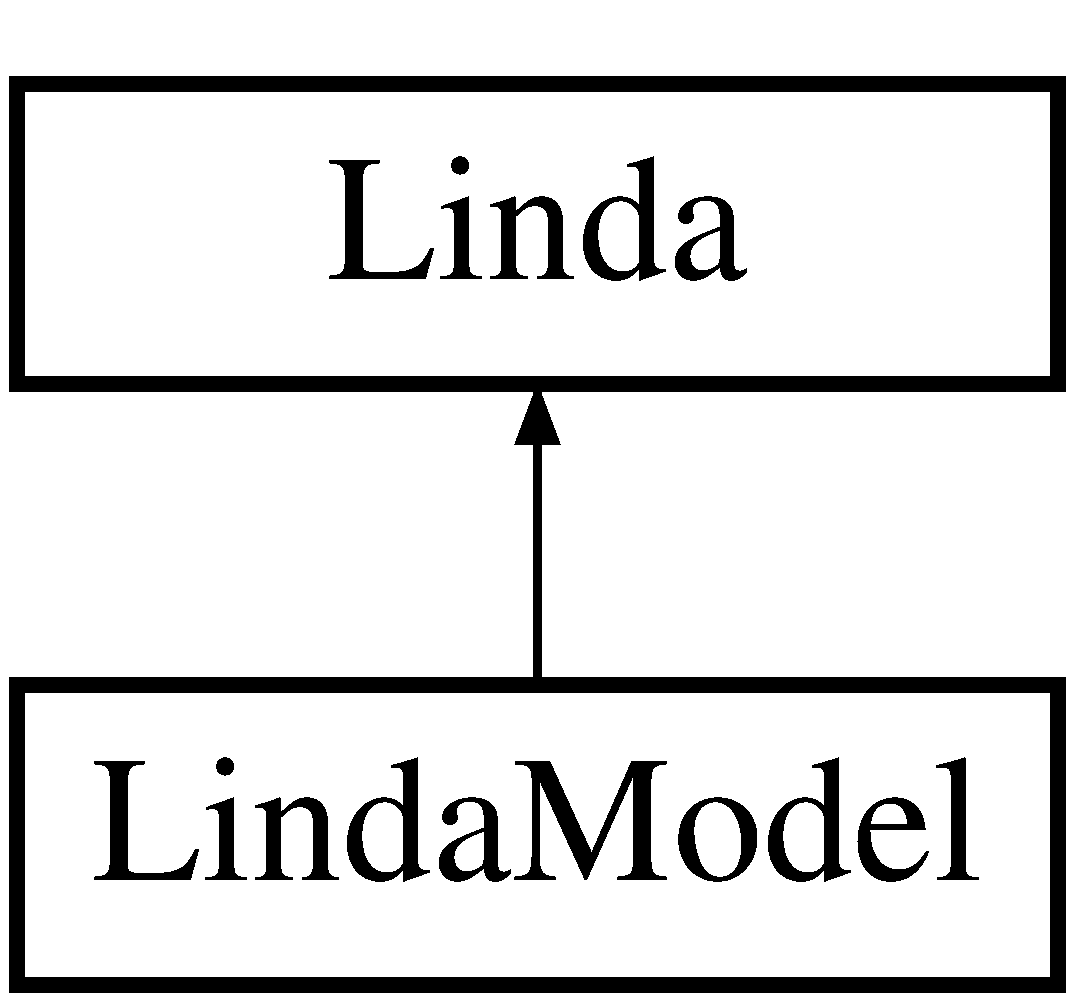
\includegraphics[height=2.000000cm]{class_linda_model}
\end{center}
\end{figure}
\subsection*{Public Member Functions}
\begin{DoxyCompactItemize}
\item 
\hyperlink{class_linda_model_a776f84c759a8aa1820e5c65719897d8d}{\+\_\+\+\_\+construct} (\$Model, \$primary\+Key=N\+U\+L\+L)
\item 
\hyperlink{class_linda_model_af008f367d5ca054454dacc1e8830d7fd}{fetch\+All} ()
\item 
\hyperlink{class_linda_model_ac73eef9ff76ea330c0dab36ca448b90d}{first} ()
\item 
\hyperlink{class_linda_model_ab24fa179a41ab9c933c32181e3d3ed84}{collection} ()
\item 
\hyperlink{class_linda_model_a637f52fa554aa09e732a30691d68e172}{save} (\$new\+\_\+flag=N\+U\+L\+L)
\item 
\hyperlink{class_linda_model_a6b574d6569f95f11d7b1ba119185ac6d}{set} (\$data=array())
\item 
\hyperlink{class_linda_model_a7acfd032bb2a094c5e81d0183f713991}{where} (\$col, \$op, \$val)
\item 
\hyperlink{class_linda_model_a4c127fc509d13b318bc343c4753617ea}{where\+\_\+or} (\$col, \$op, \$val)
\item 
\hyperlink{class_linda_model_af2cd4e8ab564012941e2e5837a64419a}{where\+\_\+in\+\_\+or} (\$col, \$val)
\item 
\hyperlink{class_linda_model_a6978f186be10e963c0bbec845bad0347}{where\+\_\+in} (\$col, \$val)
\item 
\hyperlink{class_linda_model_aadb1463eecf640b9480079f5a0862ed3}{where\+\_\+in\+\_\+numeric\+\_\+or} (\$col, \$val)
\item 
\hyperlink{class_linda_model_a89f82f99daba9a8cc4c4f5756f05054c}{where\+\_\+in\+\_\+numeric} (\$col, \$val)
\item 
\hyperlink{class_linda_model_a208a1a59285ee5a95a90c5328f3ee31e}{inner\+\_\+join} (\$table, \$conditional\+\_\+column\+\_\+a, \$conditional\+\_\+column\+\_\+b)
\item 
\hyperlink{class_linda_model_ac33ee765f5ad9f134540bac393721cfe}{get} ()
\item 
\hyperlink{class_linda_model_a65cd50a6fdf5ce1f4a0e45ab930af5fa}{skip} (\$param)
\item 
\hyperlink{class_linda_model_a33ab6a5b47dfbefa83546cab6734f017}{take} (\$param)
\item 
\hyperlink{class_linda_model_a5297010b1eb7d2cce1e0f2ad8d6d8336}{create} (\$values)
\item 
\hyperlink{class_linda_model_aff9a1fb07dca963c2c9a8ffe66b45ded}{remove} ()
\end{DoxyCompactItemize}
\subsection*{Protected Attributes}
\begin{DoxyCompactItemize}
\item 
\hyperlink{class_linda_model_a736ca8a8aaf094b1747b04f00333732c}{\$table\+Column\+Schema}
\item 
\hyperlink{class_linda_model_a1b40070fc765a8a4f2af137240160b50}{\$virtual\+Model\+Collection} = array()
\item 
\hyperlink{class_linda_model_ac155ae9a10f7fe23e69866ef520cc40a}{\$virtual\+Model\+Primary\+Key}
\item 
\hyperlink{class_linda_model_ac2d5e104b8970095b9463776a94eede0}{\$model\+Name}
\end{DoxyCompactItemize}
\subsection*{Additional Inherited Members}


\subsection{Detailed Description}
\hyperlink{class_linda_model}{Linda\+Model} is an Active-\/record based O\+R\+M, it facilitates the creation and use of business objects whose data requires persistent storage to a database. It is an implementation of the Active Record pattern which itself is a description of an Object Relational Mapping system. 

\begin{DoxyAuthor}{Author}
Olubodun Agbalaya. 
\end{DoxyAuthor}


Definition at line 15 of file Linda\+Model.\+php.



\subsection{Constructor \& Destructor Documentation}
\hypertarget{class_linda_model_a776f84c759a8aa1820e5c65719897d8d}{}\index{Linda\+Model@{Linda\+Model}!\+\_\+\+\_\+construct@{\+\_\+\+\_\+construct}}
\index{\+\_\+\+\_\+construct@{\+\_\+\+\_\+construct}!Linda\+Model@{Linda\+Model}}
\subsubsection[{\+\_\+\+\_\+construct(\$\+Model, \$primary\+Key=\+N\+U\+L\+L)}]{\setlength{\rightskip}{0pt plus 5cm}\+\_\+\+\_\+construct (
\begin{DoxyParamCaption}
\item[{}]{\$\+Model, }
\item[{}]{\$primary\+Key = {\ttfamily NULL}}
\end{DoxyParamCaption}
)}\label{class_linda_model_a776f84c759a8aa1820e5c65719897d8d}

\begin{DoxyParams}[1]{Parameters}
string & {\em \$\+Model} & The name of the table we are to create an Object Map to \\
\hline
string & {\em \$primary\+Key} & An optional primary key on the table, defaults to the first column \\
\hline
\end{DoxyParams}


Definition at line 28 of file Linda\+Model.\+php.



\subsection{Member Function Documentation}
\hypertarget{class_linda_model_ab24fa179a41ab9c933c32181e3d3ed84}{}\index{Linda\+Model@{Linda\+Model}!collection@{collection}}
\index{collection@{collection}!Linda\+Model@{Linda\+Model}}
\subsubsection[{collection()}]{\setlength{\rightskip}{0pt plus 5cm}collection (
\begin{DoxyParamCaption}
{}
\end{DoxyParamCaption}
)}\label{class_linda_model_ab24fa179a41ab9c933c32181e3d3ed84}
Returns a collections of models representing each active record, retrieved from the last call to \hyperlink{class_linda_model_ac33ee765f5ad9f134540bac393721cfe}{get} \begin{DoxyReturn}{Returns}
Linda\+Row\+Model\+Collection 
\end{DoxyReturn}


Definition at line 74 of file Linda\+Model.\+php.

\hypertarget{class_linda_model_a5297010b1eb7d2cce1e0f2ad8d6d8336}{}\index{Linda\+Model@{Linda\+Model}!create@{create}}
\index{create@{create}!Linda\+Model@{Linda\+Model}}
\subsubsection[{create(\$values)}]{\setlength{\rightskip}{0pt plus 5cm}create (
\begin{DoxyParamCaption}
\item[{}]{\$values}
\end{DoxyParamCaption}
)}\label{class_linda_model_a5297010b1eb7d2cce1e0f2ad8d6d8336}


Definition at line 194 of file Linda\+Model.\+php.

\hypertarget{class_linda_model_af008f367d5ca054454dacc1e8830d7fd}{}\index{Linda\+Model@{Linda\+Model}!fetch\+All@{fetch\+All}}
\index{fetch\+All@{fetch\+All}!Linda\+Model@{Linda\+Model}}
\subsubsection[{fetch\+All()}]{\setlength{\rightskip}{0pt plus 5cm}fetch\+All (
\begin{DoxyParamCaption}
{}
\end{DoxyParamCaption}
)}\label{class_linda_model_af008f367d5ca054454dacc1e8830d7fd}
Method to fetch all rows from the D\+B into memory, use \hyperlink{class_linda_model_ac33ee765f5ad9f134540bac393721cfe}{get} to retrieve the fields as a collection of Models \begin{DoxyReturn}{Returns}
\$this 
\end{DoxyReturn}


Definition at line 47 of file Linda\+Model.\+php.

\hypertarget{class_linda_model_ac73eef9ff76ea330c0dab36ca448b90d}{}\index{Linda\+Model@{Linda\+Model}!first@{first}}
\index{first@{first}!Linda\+Model@{Linda\+Model}}
\subsubsection[{first()}]{\setlength{\rightskip}{0pt plus 5cm}first (
\begin{DoxyParamCaption}
{}
\end{DoxyParamCaption}
)}\label{class_linda_model_ac73eef9ff76ea330c0dab36ca448b90d}
Returns first model representing an active record, or N\+U\+L\+L if no records where matched \begin{DoxyReturn}{Returns}
\hyperlink{class_linda_row_model}{Linda\+Row\+Model} 
\end{DoxyReturn}


Definition at line 65 of file Linda\+Model.\+php.

\hypertarget{class_linda_model_ac33ee765f5ad9f134540bac393721cfe}{}\index{Linda\+Model@{Linda\+Model}!get@{get}}
\index{get@{get}!Linda\+Model@{Linda\+Model}}
\subsubsection[{get()}]{\setlength{\rightskip}{0pt plus 5cm}get (
\begin{DoxyParamCaption}
{}
\end{DoxyParamCaption}
)}\label{class_linda_model_ac33ee765f5ad9f134540bac393721cfe}
Fetches data from the table based on the C\+L\+A\+U\+S\+E\+S set, and stores them in memory as distinct object models of each row/record \begin{DoxyReturn}{Returns}
\$this 
\end{DoxyReturn}


Definition at line 168 of file Linda\+Model.\+php.

\hypertarget{class_linda_model_a208a1a59285ee5a95a90c5328f3ee31e}{}\index{Linda\+Model@{Linda\+Model}!inner\+\_\+join@{inner\+\_\+join}}
\index{inner\+\_\+join@{inner\+\_\+join}!Linda\+Model@{Linda\+Model}}
\subsubsection[{inner\+\_\+join(\$table, \$conditional\+\_\+column\+\_\+a, \$conditional\+\_\+column\+\_\+b)}]{\setlength{\rightskip}{0pt plus 5cm}inner\+\_\+join (
\begin{DoxyParamCaption}
\item[{}]{\$table, }
\item[{}]{\$conditional\+\_\+column\+\_\+a, }
\item[{}]{\$conditional\+\_\+column\+\_\+b}
\end{DoxyParamCaption}
)}\label{class_linda_model_a208a1a59285ee5a95a90c5328f3ee31e}


Definition at line 158 of file Linda\+Model.\+php.

\hypertarget{class_linda_model_aff9a1fb07dca963c2c9a8ffe66b45ded}{}\index{Linda\+Model@{Linda\+Model}!remove@{remove}}
\index{remove@{remove}!Linda\+Model@{Linda\+Model}}
\subsubsection[{remove()}]{\setlength{\rightskip}{0pt plus 5cm}remove (
\begin{DoxyParamCaption}
{}
\end{DoxyParamCaption}
)}\label{class_linda_model_aff9a1fb07dca963c2c9a8ffe66b45ded}


Definition at line 210 of file Linda\+Model.\+php.

\hypertarget{class_linda_model_a637f52fa554aa09e732a30691d68e172}{}\index{Linda\+Model@{Linda\+Model}!save@{save}}
\index{save@{save}!Linda\+Model@{Linda\+Model}}
\subsubsection[{save(\$new\+\_\+flag=\+N\+U\+L\+L)}]{\setlength{\rightskip}{0pt plus 5cm}save (
\begin{DoxyParamCaption}
\item[{}]{\$new\+\_\+flag = {\ttfamily NULL}}
\end{DoxyParamCaption}
)}\label{class_linda_model_a637f52fa554aa09e732a30691d68e172}
Saves data back into the table \begin{DoxyReturn}{Returns}
\hyperlink{class_linda_row_model}{Linda\+Row\+Model}
\end{DoxyReturn}

\begin{DoxyParams}[1]{Parameters}
type & {\em \$new\+\_\+flag} & An optional primary key parameter, to use in Identfying the row to save data into \\
\hline
\end{DoxyParams}
\begin{DoxyReturn}{Returns}
$\vert$\$this 
\end{DoxyReturn}


Definition at line 87 of file Linda\+Model.\+php.

\hypertarget{class_linda_model_a6b574d6569f95f11d7b1ba119185ac6d}{}\index{Linda\+Model@{Linda\+Model}!set@{set}}
\index{set@{set}!Linda\+Model@{Linda\+Model}}
\subsubsection[{set(\$data=array())}]{\setlength{\rightskip}{0pt plus 5cm}set (
\begin{DoxyParamCaption}
\item[{}]{\$data = {\ttfamily array()}}
\end{DoxyParamCaption}
)}\label{class_linda_model_a6b574d6569f95f11d7b1ba119185ac6d}


Definition at line 114 of file Linda\+Model.\+php.

\hypertarget{class_linda_model_a65cd50a6fdf5ce1f4a0e45ab930af5fa}{}\index{Linda\+Model@{Linda\+Model}!skip@{skip}}
\index{skip@{skip}!Linda\+Model@{Linda\+Model}}
\subsubsection[{skip(\$param)}]{\setlength{\rightskip}{0pt plus 5cm}skip (
\begin{DoxyParamCaption}
\item[{}]{\$param}
\end{DoxyParamCaption}
)}\label{class_linda_model_a65cd50a6fdf5ce1f4a0e45ab930af5fa}


Definition at line 181 of file Linda\+Model.\+php.

\hypertarget{class_linda_model_a33ab6a5b47dfbefa83546cab6734f017}{}\index{Linda\+Model@{Linda\+Model}!take@{take}}
\index{take@{take}!Linda\+Model@{Linda\+Model}}
\subsubsection[{take(\$param)}]{\setlength{\rightskip}{0pt plus 5cm}take (
\begin{DoxyParamCaption}
\item[{}]{\$param}
\end{DoxyParamCaption}
)}\label{class_linda_model_a33ab6a5b47dfbefa83546cab6734f017}


Definition at line 188 of file Linda\+Model.\+php.

\hypertarget{class_linda_model_a7acfd032bb2a094c5e81d0183f713991}{}\index{Linda\+Model@{Linda\+Model}!where@{where}}
\index{where@{where}!Linda\+Model@{Linda\+Model}}
\subsubsection[{where(\$col, \$op, \$val)}]{\setlength{\rightskip}{0pt plus 5cm}where (
\begin{DoxyParamCaption}
\item[{}]{\$col, }
\item[{}]{\$op, }
\item[{}]{\$val}
\end{DoxyParamCaption}
)}\label{class_linda_model_a7acfd032bb2a094c5e81d0183f713991}


Definition at line 124 of file Linda\+Model.\+php.

\hypertarget{class_linda_model_a6978f186be10e963c0bbec845bad0347}{}\index{Linda\+Model@{Linda\+Model}!where\+\_\+in@{where\+\_\+in}}
\index{where\+\_\+in@{where\+\_\+in}!Linda\+Model@{Linda\+Model}}
\subsubsection[{where\+\_\+in(\$col, \$val)}]{\setlength{\rightskip}{0pt plus 5cm}where\+\_\+in (
\begin{DoxyParamCaption}
\item[{}]{\$col, }
\item[{}]{\$val}
\end{DoxyParamCaption}
)}\label{class_linda_model_a6978f186be10e963c0bbec845bad0347}


Definition at line 140 of file Linda\+Model.\+php.

\hypertarget{class_linda_model_a89f82f99daba9a8cc4c4f5756f05054c}{}\index{Linda\+Model@{Linda\+Model}!where\+\_\+in\+\_\+numeric@{where\+\_\+in\+\_\+numeric}}
\index{where\+\_\+in\+\_\+numeric@{where\+\_\+in\+\_\+numeric}!Linda\+Model@{Linda\+Model}}
\subsubsection[{where\+\_\+in\+\_\+numeric(\$col, \$val)}]{\setlength{\rightskip}{0pt plus 5cm}where\+\_\+in\+\_\+numeric (
\begin{DoxyParamCaption}
\item[{}]{\$col, }
\item[{}]{\$val}
\end{DoxyParamCaption}
)}\label{class_linda_model_a89f82f99daba9a8cc4c4f5756f05054c}


Definition at line 152 of file Linda\+Model.\+php.

\hypertarget{class_linda_model_aadb1463eecf640b9480079f5a0862ed3}{}\index{Linda\+Model@{Linda\+Model}!where\+\_\+in\+\_\+numeric\+\_\+or@{where\+\_\+in\+\_\+numeric\+\_\+or}}
\index{where\+\_\+in\+\_\+numeric\+\_\+or@{where\+\_\+in\+\_\+numeric\+\_\+or}!Linda\+Model@{Linda\+Model}}
\subsubsection[{where\+\_\+in\+\_\+numeric\+\_\+or(\$col, \$val)}]{\setlength{\rightskip}{0pt plus 5cm}where\+\_\+in\+\_\+numeric\+\_\+or (
\begin{DoxyParamCaption}
\item[{}]{\$col, }
\item[{}]{\$val}
\end{DoxyParamCaption}
)}\label{class_linda_model_aadb1463eecf640b9480079f5a0862ed3}


Definition at line 146 of file Linda\+Model.\+php.

\hypertarget{class_linda_model_af2cd4e8ab564012941e2e5837a64419a}{}\index{Linda\+Model@{Linda\+Model}!where\+\_\+in\+\_\+or@{where\+\_\+in\+\_\+or}}
\index{where\+\_\+in\+\_\+or@{where\+\_\+in\+\_\+or}!Linda\+Model@{Linda\+Model}}
\subsubsection[{where\+\_\+in\+\_\+or(\$col, \$val)}]{\setlength{\rightskip}{0pt plus 5cm}where\+\_\+in\+\_\+or (
\begin{DoxyParamCaption}
\item[{}]{\$col, }
\item[{}]{\$val}
\end{DoxyParamCaption}
)}\label{class_linda_model_af2cd4e8ab564012941e2e5837a64419a}


Definition at line 134 of file Linda\+Model.\+php.

\hypertarget{class_linda_model_a4c127fc509d13b318bc343c4753617ea}{}\index{Linda\+Model@{Linda\+Model}!where\+\_\+or@{where\+\_\+or}}
\index{where\+\_\+or@{where\+\_\+or}!Linda\+Model@{Linda\+Model}}
\subsubsection[{where\+\_\+or(\$col, \$op, \$val)}]{\setlength{\rightskip}{0pt plus 5cm}where\+\_\+or (
\begin{DoxyParamCaption}
\item[{}]{\$col, }
\item[{}]{\$op, }
\item[{}]{\$val}
\end{DoxyParamCaption}
)}\label{class_linda_model_a4c127fc509d13b318bc343c4753617ea}


Definition at line 129 of file Linda\+Model.\+php.



\subsection{Field Documentation}
\hypertarget{class_linda_model_ac2d5e104b8970095b9463776a94eede0}{}\index{Linda\+Model@{Linda\+Model}!\$model\+Name@{\$model\+Name}}
\index{\$model\+Name@{\$model\+Name}!Linda\+Model@{Linda\+Model}}
\subsubsection[{\$model\+Name}]{\setlength{\rightskip}{0pt plus 5cm}\$model\+Name\hspace{0.3cm}{\ttfamily [protected]}}\label{class_linda_model_ac2d5e104b8970095b9463776a94eede0}


Definition at line 20 of file Linda\+Model.\+php.

\hypertarget{class_linda_model_a736ca8a8aaf094b1747b04f00333732c}{}\index{Linda\+Model@{Linda\+Model}!\$table\+Column\+Schema@{\$table\+Column\+Schema}}
\index{\$table\+Column\+Schema@{\$table\+Column\+Schema}!Linda\+Model@{Linda\+Model}}
\subsubsection[{\$table\+Column\+Schema}]{\setlength{\rightskip}{0pt plus 5cm}\$table\+Column\+Schema\hspace{0.3cm}{\ttfamily [protected]}}\label{class_linda_model_a736ca8a8aaf094b1747b04f00333732c}


Definition at line 17 of file Linda\+Model.\+php.

\hypertarget{class_linda_model_a1b40070fc765a8a4f2af137240160b50}{}\index{Linda\+Model@{Linda\+Model}!\$virtual\+Model\+Collection@{\$virtual\+Model\+Collection}}
\index{\$virtual\+Model\+Collection@{\$virtual\+Model\+Collection}!Linda\+Model@{Linda\+Model}}
\subsubsection[{\$virtual\+Model\+Collection}]{\setlength{\rightskip}{0pt plus 5cm}\$virtual\+Model\+Collection = array()\hspace{0.3cm}{\ttfamily [protected]}}\label{class_linda_model_a1b40070fc765a8a4f2af137240160b50}


Definition at line 18 of file Linda\+Model.\+php.

\hypertarget{class_linda_model_ac155ae9a10f7fe23e69866ef520cc40a}{}\index{Linda\+Model@{Linda\+Model}!\$virtual\+Model\+Primary\+Key@{\$virtual\+Model\+Primary\+Key}}
\index{\$virtual\+Model\+Primary\+Key@{\$virtual\+Model\+Primary\+Key}!Linda\+Model@{Linda\+Model}}
\subsubsection[{\$virtual\+Model\+Primary\+Key}]{\setlength{\rightskip}{0pt plus 5cm}\$virtual\+Model\+Primary\+Key\hspace{0.3cm}{\ttfamily [protected]}}\label{class_linda_model_ac155ae9a10f7fe23e69866ef520cc40a}


Definition at line 19 of file Linda\+Model.\+php.



The documentation for this class was generated from the following file\+:\begin{DoxyCompactItemize}
\item 
C\+:/\+Apache24/htdocs/easygo/process/\+Linda/\hyperlink{_linda_model_8php}{Linda\+Model.\+php}\end{DoxyCompactItemize}

\hypertarget{class_linda_row_model}{}\section{Linda\+Row\+Model Class Reference}
\label{class_linda_row_model}\index{Linda\+Row\+Model@{Linda\+Row\+Model}}
\subsection*{Public Member Functions}
\begin{DoxyCompactItemize}
\item 
\hyperlink{class_linda_row_model_ad0a8f6d6175503438e94bc49123f8347}{\+\_\+\+\_\+construct} (\$column, \$data)
\item 
\hyperlink{class_linda_row_model_abc8e9e31bb15c8a44c3210ec551407c8}{\+\_\+\+\_\+get} (\$name)
\item 
\hyperlink{class_linda_row_model_a83c2703c91959192f759992ad5640b67}{\+\_\+\+\_\+set} (\$name, \$value)
\item 
\hyperlink{class_linda_row_model_abb1240d4b8d4521d783a58d9b1f1df0a}{has\+Key} (\$name)
\item 
\hyperlink{class_linda_row_model_a70a0fe08035189260c72e32a9e20d30c}{get\+Values} ()
\item 
\hyperlink{class_linda_row_model_aa21c070bc4453dc79caa7f30a53ea7a2}{get\+Values\+As\+Object} ()
\item 
\hyperlink{class_linda_row_model_a421831a265621325e1fdd19aace0c758}{\+\_\+\+\_\+destruct} ()
\end{DoxyCompactItemize}


\subsection{Detailed Description}


Definition at line 3 of file Linda\+Row\+Model.\+php.



\subsection{Constructor \& Destructor Documentation}
\hypertarget{class_linda_row_model_ad0a8f6d6175503438e94bc49123f8347}{}\index{Linda\+Row\+Model@{Linda\+Row\+Model}!\+\_\+\+\_\+construct@{\+\_\+\+\_\+construct}}
\index{\+\_\+\+\_\+construct@{\+\_\+\+\_\+construct}!Linda\+Row\+Model@{Linda\+Row\+Model}}
\subsubsection[{\+\_\+\+\_\+construct(\$column, \$data)}]{\setlength{\rightskip}{0pt plus 5cm}\+\_\+\+\_\+construct (
\begin{DoxyParamCaption}
\item[{}]{\$column, }
\item[{}]{\$data}
\end{DoxyParamCaption}
)}\label{class_linda_row_model_ad0a8f6d6175503438e94bc49123f8347}


Definition at line 8 of file Linda\+Row\+Model.\+php.

\hypertarget{class_linda_row_model_a421831a265621325e1fdd19aace0c758}{}\index{Linda\+Row\+Model@{Linda\+Row\+Model}!\+\_\+\+\_\+destruct@{\+\_\+\+\_\+destruct}}
\index{\+\_\+\+\_\+destruct@{\+\_\+\+\_\+destruct}!Linda\+Row\+Model@{Linda\+Row\+Model}}
\subsubsection[{\+\_\+\+\_\+destruct()}]{\setlength{\rightskip}{0pt plus 5cm}\+\_\+\+\_\+destruct (
\begin{DoxyParamCaption}
{}
\end{DoxyParamCaption}
)}\label{class_linda_row_model_a421831a265621325e1fdd19aace0c758}


Definition at line 58 of file Linda\+Row\+Model.\+php.



\subsection{Member Function Documentation}
\hypertarget{class_linda_row_model_abc8e9e31bb15c8a44c3210ec551407c8}{}\index{Linda\+Row\+Model@{Linda\+Row\+Model}!\+\_\+\+\_\+get@{\+\_\+\+\_\+get}}
\index{\+\_\+\+\_\+get@{\+\_\+\+\_\+get}!Linda\+Row\+Model@{Linda\+Row\+Model}}
\subsubsection[{\+\_\+\+\_\+get(\$name)}]{\setlength{\rightskip}{0pt plus 5cm}\+\_\+\+\_\+get (
\begin{DoxyParamCaption}
\item[{}]{\$name}
\end{DoxyParamCaption}
)}\label{class_linda_row_model_abc8e9e31bb15c8a44c3210ec551407c8}


Definition at line 18 of file Linda\+Row\+Model.\+php.

\hypertarget{class_linda_row_model_a83c2703c91959192f759992ad5640b67}{}\index{Linda\+Row\+Model@{Linda\+Row\+Model}!\+\_\+\+\_\+set@{\+\_\+\+\_\+set}}
\index{\+\_\+\+\_\+set@{\+\_\+\+\_\+set}!Linda\+Row\+Model@{Linda\+Row\+Model}}
\subsubsection[{\+\_\+\+\_\+set(\$name, \$value)}]{\setlength{\rightskip}{0pt plus 5cm}\+\_\+\+\_\+set (
\begin{DoxyParamCaption}
\item[{}]{\$name, }
\item[{}]{\$value}
\end{DoxyParamCaption}
)}\label{class_linda_row_model_a83c2703c91959192f759992ad5640b67}


Definition at line 27 of file Linda\+Row\+Model.\+php.

\hypertarget{class_linda_row_model_a70a0fe08035189260c72e32a9e20d30c}{}\index{Linda\+Row\+Model@{Linda\+Row\+Model}!get\+Values@{get\+Values}}
\index{get\+Values@{get\+Values}!Linda\+Row\+Model@{Linda\+Row\+Model}}
\subsubsection[{get\+Values()}]{\setlength{\rightskip}{0pt plus 5cm}get\+Values (
\begin{DoxyParamCaption}
{}
\end{DoxyParamCaption}
)}\label{class_linda_row_model_a70a0fe08035189260c72e32a9e20d30c}


Definition at line 45 of file Linda\+Row\+Model.\+php.

\hypertarget{class_linda_row_model_aa21c070bc4453dc79caa7f30a53ea7a2}{}\index{Linda\+Row\+Model@{Linda\+Row\+Model}!get\+Values\+As\+Object@{get\+Values\+As\+Object}}
\index{get\+Values\+As\+Object@{get\+Values\+As\+Object}!Linda\+Row\+Model@{Linda\+Row\+Model}}
\subsubsection[{get\+Values\+As\+Object()}]{\setlength{\rightskip}{0pt plus 5cm}get\+Values\+As\+Object (
\begin{DoxyParamCaption}
{}
\end{DoxyParamCaption}
)}\label{class_linda_row_model_aa21c070bc4453dc79caa7f30a53ea7a2}


Definition at line 49 of file Linda\+Row\+Model.\+php.

\hypertarget{class_linda_row_model_abb1240d4b8d4521d783a58d9b1f1df0a}{}\index{Linda\+Row\+Model@{Linda\+Row\+Model}!has\+Key@{has\+Key}}
\index{has\+Key@{has\+Key}!Linda\+Row\+Model@{Linda\+Row\+Model}}
\subsubsection[{has\+Key(\$name)}]{\setlength{\rightskip}{0pt plus 5cm}has\+Key (
\begin{DoxyParamCaption}
\item[{}]{\$name}
\end{DoxyParamCaption}
)}\label{class_linda_row_model_abb1240d4b8d4521d783a58d9b1f1df0a}


Definition at line 37 of file Linda\+Row\+Model.\+php.



The documentation for this class was generated from the following file\+:\begin{DoxyCompactItemize}
\item 
C\+:/\+Apache24/htdocs/easygo/process/\+Linda/\hyperlink{_linda_row_model_8php}{Linda\+Row\+Model.\+php}\end{DoxyCompactItemize}

\chapter{File Documentation}
\hypertarget{_linda_8inc}{}\section{C\+:/\+Apache24/htdocs/easygo/process/\+Linda/\+Linda.inc File Reference}
\label{_linda_8inc}\index{C\+:/\+Apache24/htdocs/easygo/process/\+Linda/\+Linda.\+inc@{C\+:/\+Apache24/htdocs/easygo/process/\+Linda/\+Linda.\+inc}}
\subsection*{Variables}
\begin{DoxyCompactItemize}
\item 
const \hyperlink{_linda_8inc_a86b40c589d474db371ea58296a5eeb12}{L\+I\+N\+D\+A\+\_\+\+D\+B\+\_\+\+H\+O\+S\+T} \textquotesingle{}localhost\textquotesingle{}
\item 
const \hyperlink{_linda_8inc_a75c0048bcb27b8bf9d4e9fd1b9eb023b}{L\+I\+N\+D\+A\+\_\+\+D\+B\+\_\+\+T\+Y\+P\+E} \textquotesingle{}mysql\textquotesingle{}
\item 
const \hyperlink{_linda_8inc_a4e480c562d1f6701e89f603607ddbb54}{L\+I\+N\+D\+A\+\_\+\+D\+B\+\_\+\+N\+A\+M\+E} \textquotesingle{}egown\+\_\+db\textquotesingle{}
\item 
const \hyperlink{_linda_8inc_a713707c7fea371f7f3892136c1e852f0}{L\+I\+N\+D\+A\+\_\+\+D\+B\+\_\+\+U\+S\+E\+R} \textquotesingle{}easygow\+\_\+user\textquotesingle{}
\item 
const \hyperlink{_linda_8inc_aef9b254dff90502b875151a93b462df1}{L\+I\+N\+D\+A\+\_\+\+D\+B\+\_\+\+P\+A\+S\+S\+W} \textquotesingle{}easygow\+\_\+secure\textquotesingle{}
\end{DoxyCompactItemize}


\subsection{Variable Documentation}
\hypertarget{_linda_8inc_a86b40c589d474db371ea58296a5eeb12}{}\index{Linda.\+inc@{Linda.\+inc}!L\+I\+N\+D\+A\+\_\+\+D\+B\+\_\+\+H\+O\+S\+T@{L\+I\+N\+D\+A\+\_\+\+D\+B\+\_\+\+H\+O\+S\+T}}
\index{L\+I\+N\+D\+A\+\_\+\+D\+B\+\_\+\+H\+O\+S\+T@{L\+I\+N\+D\+A\+\_\+\+D\+B\+\_\+\+H\+O\+S\+T}!Linda.\+inc@{Linda.\+inc}}
\subsubsection[{L\+I\+N\+D\+A\+\_\+\+D\+B\+\_\+\+H\+O\+S\+T}]{\setlength{\rightskip}{0pt plus 5cm}const L\+I\+N\+D\+A\+\_\+\+D\+B\+\_\+\+H\+O\+S\+T \textquotesingle{}localhost\textquotesingle{}}\label{_linda_8inc_a86b40c589d474db371ea58296a5eeb12}
\begin{Desc}
\item[Examples\+: ]\par
\hyperlink{_c_1_2_apache24_2htdocs_2easygo_2process_2_linda_2_linda_8php-example}{C\+:/\+Apache24/htdocs/easygo/process/\+Linda/\+Linda.\+php}.\end{Desc}


Definition at line 4 of file Linda.\+inc.

\hypertarget{_linda_8inc_a4e480c562d1f6701e89f603607ddbb54}{}\index{Linda.\+inc@{Linda.\+inc}!L\+I\+N\+D\+A\+\_\+\+D\+B\+\_\+\+N\+A\+M\+E@{L\+I\+N\+D\+A\+\_\+\+D\+B\+\_\+\+N\+A\+M\+E}}
\index{L\+I\+N\+D\+A\+\_\+\+D\+B\+\_\+\+N\+A\+M\+E@{L\+I\+N\+D\+A\+\_\+\+D\+B\+\_\+\+N\+A\+M\+E}!Linda.\+inc@{Linda.\+inc}}
\subsubsection[{L\+I\+N\+D\+A\+\_\+\+D\+B\+\_\+\+N\+A\+M\+E}]{\setlength{\rightskip}{0pt plus 5cm}const L\+I\+N\+D\+A\+\_\+\+D\+B\+\_\+\+N\+A\+M\+E \textquotesingle{}egown\+\_\+db\textquotesingle{}}\label{_linda_8inc_a4e480c562d1f6701e89f603607ddbb54}
\begin{Desc}
\item[Examples\+: ]\par
\hyperlink{_c_1_2_apache24_2htdocs_2easygo_2process_2_linda_2_linda_8php-example}{C\+:/\+Apache24/htdocs/easygo/process/\+Linda/\+Linda.\+php}.\end{Desc}


Definition at line 6 of file Linda.\+inc.

\hypertarget{_linda_8inc_aef9b254dff90502b875151a93b462df1}{}\index{Linda.\+inc@{Linda.\+inc}!L\+I\+N\+D\+A\+\_\+\+D\+B\+\_\+\+P\+A\+S\+S\+W@{L\+I\+N\+D\+A\+\_\+\+D\+B\+\_\+\+P\+A\+S\+S\+W}}
\index{L\+I\+N\+D\+A\+\_\+\+D\+B\+\_\+\+P\+A\+S\+S\+W@{L\+I\+N\+D\+A\+\_\+\+D\+B\+\_\+\+P\+A\+S\+S\+W}!Linda.\+inc@{Linda.\+inc}}
\subsubsection[{L\+I\+N\+D\+A\+\_\+\+D\+B\+\_\+\+P\+A\+S\+S\+W}]{\setlength{\rightskip}{0pt plus 5cm}const L\+I\+N\+D\+A\+\_\+\+D\+B\+\_\+\+P\+A\+S\+S\+W \textquotesingle{}easygow\+\_\+secure\textquotesingle{}}\label{_linda_8inc_aef9b254dff90502b875151a93b462df1}
\begin{Desc}
\item[Examples\+: ]\par
\hyperlink{_c_1_2_apache24_2htdocs_2easygo_2process_2_linda_2_linda_8php-example}{C\+:/\+Apache24/htdocs/easygo/process/\+Linda/\+Linda.\+php}.\end{Desc}


Definition at line 8 of file Linda.\+inc.

\hypertarget{_linda_8inc_a75c0048bcb27b8bf9d4e9fd1b9eb023b}{}\index{Linda.\+inc@{Linda.\+inc}!L\+I\+N\+D\+A\+\_\+\+D\+B\+\_\+\+T\+Y\+P\+E@{L\+I\+N\+D\+A\+\_\+\+D\+B\+\_\+\+T\+Y\+P\+E}}
\index{L\+I\+N\+D\+A\+\_\+\+D\+B\+\_\+\+T\+Y\+P\+E@{L\+I\+N\+D\+A\+\_\+\+D\+B\+\_\+\+T\+Y\+P\+E}!Linda.\+inc@{Linda.\+inc}}
\subsubsection[{L\+I\+N\+D\+A\+\_\+\+D\+B\+\_\+\+T\+Y\+P\+E}]{\setlength{\rightskip}{0pt plus 5cm}const L\+I\+N\+D\+A\+\_\+\+D\+B\+\_\+\+T\+Y\+P\+E \textquotesingle{}mysql\textquotesingle{}}\label{_linda_8inc_a75c0048bcb27b8bf9d4e9fd1b9eb023b}
\begin{Desc}
\item[Examples\+: ]\par
\hyperlink{_c_1_2_apache24_2htdocs_2easygo_2process_2_linda_2_linda_8php-example}{C\+:/\+Apache24/htdocs/easygo/process/\+Linda/\+Linda.\+php}.\end{Desc}


Definition at line 5 of file Linda.\+inc.

\hypertarget{_linda_8inc_a713707c7fea371f7f3892136c1e852f0}{}\index{Linda.\+inc@{Linda.\+inc}!L\+I\+N\+D\+A\+\_\+\+D\+B\+\_\+\+U\+S\+E\+R@{L\+I\+N\+D\+A\+\_\+\+D\+B\+\_\+\+U\+S\+E\+R}}
\index{L\+I\+N\+D\+A\+\_\+\+D\+B\+\_\+\+U\+S\+E\+R@{L\+I\+N\+D\+A\+\_\+\+D\+B\+\_\+\+U\+S\+E\+R}!Linda.\+inc@{Linda.\+inc}}
\subsubsection[{L\+I\+N\+D\+A\+\_\+\+D\+B\+\_\+\+U\+S\+E\+R}]{\setlength{\rightskip}{0pt plus 5cm}const L\+I\+N\+D\+A\+\_\+\+D\+B\+\_\+\+U\+S\+E\+R \textquotesingle{}easygow\+\_\+user\textquotesingle{}}\label{_linda_8inc_a713707c7fea371f7f3892136c1e852f0}
\begin{Desc}
\item[Examples\+: ]\par
\hyperlink{_c_1_2_apache24_2htdocs_2easygo_2process_2_linda_2_linda_8php-example}{C\+:/\+Apache24/htdocs/easygo/process/\+Linda/\+Linda.\+php}.\end{Desc}


Definition at line 7 of file Linda.\+inc.


\hypertarget{_linda_8php}{}\section{C\+:/\+Apache24/htdocs/easygo/process/\+Linda/\+Linda.php File Reference}
\label{_linda_8php}\index{C\+:/\+Apache24/htdocs/easygo/process/\+Linda/\+Linda.\+php@{C\+:/\+Apache24/htdocs/easygo/process/\+Linda/\+Linda.\+php}}
\subsection*{Data Structures}
\begin{DoxyCompactItemize}
\item 
class \hyperlink{class_linda}{Linda}
\begin{DoxyCompactList}\small\item\em \hyperlink{class_linda}{Linda} is a Database Abstraction Layer for P\+H\+P Built on top P\+D\+O. \end{DoxyCompactList}\end{DoxyCompactItemize}

\hypertarget{_linda_model_8php}{}\section{C\+:/\+Apache24/htdocs/easygo/process/\+Linda/\+Linda\+Model.php File Reference}
\label{_linda_model_8php}\index{C\+:/\+Apache24/htdocs/easygo/process/\+Linda/\+Linda\+Model.\+php@{C\+:/\+Apache24/htdocs/easygo/process/\+Linda/\+Linda\+Model.\+php}}
\subsection*{Data Structures}
\begin{DoxyCompactItemize}
\item 
class \hyperlink{class_linda_model}{Linda\+Model}
\begin{DoxyCompactList}\small\item\em \hyperlink{class_linda_model}{Linda\+Model} is an Active-\/record based O\+R\+M, it facilitates the creation and use of business objects whose data requires persistent storage to a database. It is an implementation of the Active Record pattern which itself is a description of an Object Relational Mapping system. \end{DoxyCompactList}\end{DoxyCompactItemize}

\hypertarget{_linda_row_model_8php}{}\section{C\+:/\+Apache24/htdocs/easygo/process/\+Linda/\+Linda\+Row\+Model.php File Reference}
\label{_linda_row_model_8php}\index{C\+:/\+Apache24/htdocs/easygo/process/\+Linda/\+Linda\+Row\+Model.\+php@{C\+:/\+Apache24/htdocs/easygo/process/\+Linda/\+Linda\+Row\+Model.\+php}}
\subsection*{Data Structures}
\begin{DoxyCompactItemize}
\item 
class \hyperlink{class_linda_row_model}{Linda\+Row\+Model}
\end{DoxyCompactItemize}

\chapter{Example Documentation}
\hypertarget{_c_1_2_apache24_2htdocs_2easygo_2process_2_linda_2_linda_8php-example}{}\section{C\+:/\+Apache24/htdocs/easygo/process/\+Linda/\+Linda.\+php}
Update fields in the D\+B


\begin{DoxyParams}[1]{Parameters}
Array & {\em \$fields} & is an associative array containing values to set\\
\hline
\end{DoxyParams}
\$fields = array( id= \char`\"{}1\char`\"{}, email = "example.\+example.\+org ) using N\+O\+W() or T\+I\+M\+E() as values, inserts the date/time 
\begin{DoxyParams}[1]{Parameters}
type & {\em \$query\+Config,see} & \#insert for structure of the query\+Config parameter\\
\hline
\end{DoxyParams}

\begin{DoxyCodeInclude}
<?php


include\_once $\_SERVER[\textcolor{stringliteral}{'DOCUMENT\_ROOT'}] . \textcolor{stringliteral}{'/process/Linda/Linda.inc'};

\textcolor{keyword}{class }\hyperlink{class_linda}{Linda} \{

    \textcolor{keyword}{public} \hyperlink{class_linda_ab7d7da38a7a04e1f95bc46697f8d80e3}{$LINDA\_ERROR} = NULL;
    \textcolor{keyword}{protected} \hyperlink{class_linda_a11c2781ac527a1c951d9035f2d0197cc}{$DB\_LINK};
    \textcolor{keyword}{protected} \hyperlink{class_linda_a486c281995ea6cdb9fb0367b6e260b76}{$TABLE\_MODEL};
    \textcolor{keyword}{public} \hyperlink{class_linda_a5ed9b689dc54a1e48103d904af6885a5}{$CURRENT\_QUERY};
    \textcolor{keyword}{protected} \hyperlink{class_linda_a46c628c6bd56ec5880da2515cf352183}{$MODEL\_SCHEMA} = array();
    \textcolor{keyword}{protected} \hyperlink{class_linda_a97365f1875db5efbdefc5faa71249ff1}{$DEFAULT\_LIMIT} = 1000;
    \textcolor{keyword}{protected} \hyperlink{class_linda_a803cce07cc3e3f9937b6e5faba4100fe}{$DEFAULT\_START\_INDEX} = 0;
    \textcolor{keyword}{protected} \hyperlink{class_linda_a64270a514fbca17fe7347df6320fc4ba}{$resultObject} = NULL;
    \textcolor{keyword}{protected} \hyperlink{class_linda_a038edab690e03aff9c70a1f63c06f27e}{$lastAffectedRowCount} = 0;
    \textcolor{keyword}{protected} \hyperlink{class_linda_aea7d038e46660f55592569906cf09494}{$queryConfig} = array();

    \textcolor{keyword}{const} \hyperlink{class_linda_a4771733014ade9011a85f4d01b24f2fe}{Linda\_DB\_HOST} = \hyperlink{_linda_8inc_a86b40c589d474db371ea58296a5eeb12}{LINDA\_DB\_HOST};
    \textcolor{keyword}{const} \hyperlink{class_linda_aab80e54270eaebb370e54ec5232be43a}{Linda\_DB\_NAME} = \hyperlink{_linda_8inc_a4e480c562d1f6701e89f603607ddbb54}{LINDA\_DB\_NAME};
    \textcolor{keyword}{const} \hyperlink{class_linda_af392abe38a40b56515eb835fa3c39d8c}{Linda\_DB\_TYPE} = \hyperlink{_linda_8inc_a75c0048bcb27b8bf9d4e9fd1b9eb023b}{LINDA\_DB\_TYPE};
    \textcolor{keyword}{const} \hyperlink{class_linda_a73fe432dd03d1c21aa74940da5c04dc0}{Linda\_DB\_USER} = \hyperlink{_linda_8inc_a713707c7fea371f7f3892136c1e852f0}{LINDA\_DB\_USER};
    \textcolor{keyword}{const} \hyperlink{class_linda_a392451b719cb6bb9b0c372832ad9e6d8}{Linda\_DB\_PASSW} = \hyperlink{_linda_8inc_aef9b254dff90502b875151a93b462df1}{LINDA\_DB\_PASSW};

    \textcolor{keyword}{public} \textcolor{keyword}{function} \hyperlink{class_linda_a095c5d389db211932136b53f25f39685}{\_\_construct}() \{

        $this->initConnnection();
    \}

    \textcolor{keyword}{public} \textcolor{keyword}{function} \hyperlink{class_linda_aaded27ecadbc8530b9b21cbb38dfa4a8}{setTable}($tableName) \{


        \textcolor{keywordflow}{if} (is\_string($tableName))
            $this->TABLE\_MODEL = $tableName;
    \}

    \textcolor{comment}{//+========================================================================================}
    \textcolor{keyword}{protected} \textcolor{keyword}{function} \hyperlink{class_linda_a3749f401c64588bfbecbcc3b2c1a24e4}{parseModel}() \{


        $sql = \textcolor{stringliteral}{"SELECT COLUMN\_NAME FROM INFORMATION\_SCHEMA.COLUMNS WHERE table\_name = :table"};
        \textcolor{keywordflow}{try} \{
            $core = \hyperlink{class_linda_a11c2781ac527a1c951d9035f2d0197cc}{$this->DB\_LINK};
            $stmt = $core->prepare($sql);
            $stmt->bindValue(\textcolor{stringliteral}{':table'}, $this->TABLE\_MODEL, PDO::PARAM\_STR);
            $stmt->execute();

            \textcolor{keywordflow}{while} ($row = $stmt->fetch(PDO::FETCH\_ASSOC)) \{
                $this->MODEL\_SCHEMA[] = $row[\textcolor{stringliteral}{'COLUMN\_NAME'}];
            \}
            \textcolor{keywordflow}{return} \hyperlink{class_linda_a46c628c6bd56ec5880da2515cf352183}{$this->MODEL\_SCHEMA};
        \} \textcolor{keywordflow}{catch} (PDOException $pe) \{
            trigger\_error(\textcolor{stringliteral}{'Could not connect to MySQL database. '} . $pe->getMessage(), E\_USER\_ERROR);
        \}
    \}

\textcolor{comment}{//
      +=========================================================================================================}
\textcolor{comment}{}    \textcolor{keyword}{private} \textcolor{keyword}{function} initConnnection() \{
        \textcolor{keywordflow}{try} \{
            $this->DB\_LINK = \textcolor{keyword}{new} PDO(self::Linda\_DB\_TYPE . \textcolor{stringliteral}{':host='} . self::Linda\_DB\_HOST . \textcolor{stringliteral}{';dbname='} . 
      self::Linda\_DB\_NAME, self::Linda\_DB\_USER, self::Linda\_DB\_PASSW, array(PDO::ATTR\_PERSISTENT => \textcolor{keyword}{true}));

            $this->DB\_LINK->setAttribute(PDO::ATTR\_ERRMODE, PDO::ERRMODE\_EXCEPTION);

            \textcolor{keywordflow}{return} TRUE;
        \} \textcolor{keywordflow}{catch} (PDOException $pe) \{
            $this->\hyperlink{class_linda_ab7d7da38a7a04e1f95bc46697f8d80e3}{$LINDA\_ERROR} = \textcolor{stringliteral}{"DB\_CONNECT\_ERROR"};
            \textcolor{keywordflow}{throw} $pe;
        \}
    \}

\textcolor{comment}{//
      +=========================================================================================================}

    \textcolor{keyword}{public} \textcolor{keyword}{function} \hyperlink{class_linda_a87d58413379d402e5dee4f5825b686fd}{fetch}($fields, \hyperlink{class_linda_aea7d038e46660f55592569906cf09494}{$queryConfig} = array()) \{

        $this->resultObject = null;
        $this->\hyperlink{class_linda_aeb66ebf99ca730ea67c612735a6576b4}{queryBuilder}(\textcolor{stringliteral}{"select"}, $fields, \hyperlink{class_linda_aea7d038e46660f55592569906cf09494}{$queryConfig});

        $this->\hyperlink{class_linda_ad2e4fa0b57c9acdf15cd932346381af5}{runQuery}();
        \textcolor{keywordflow}{return} $this;
    \}

    \textcolor{comment}{//
      +=========================================================================================================}

    \textcolor{keyword}{public} \textcolor{keyword}{function} \hyperlink{class_linda_ac000dfba7a410bb147dc77571d1e2ed5}{update}($fields, \hyperlink{class_linda_aea7d038e46660f55592569906cf09494}{$queryConfig}) \{
        $this->resultObject = NULL;

        $this->\hyperlink{class_linda_aeb66ebf99ca730ea67c612735a6576b4}{queryBuilder}(\textcolor{stringliteral}{"update"}, $fields, \hyperlink{class_linda_aea7d038e46660f55592569906cf09494}{$queryConfig});
        $this->\hyperlink{class_linda_ad2e4fa0b57c9acdf15cd932346381af5}{runQuery}();

        \textcolor{keywordflow}{return} $this;
    \}

    \textcolor{comment}{//
      +=========================================================================================================}
\textcolor{comment}{}    \textcolor{keyword}{public} \textcolor{keyword}{function} \hyperlink{class_linda_af5a8f159a27ca700aa869092a5696be1}{put}($fields, $values) \{

        $this->resultObject = NULL;
        $this->\hyperlink{class_linda_a190c686da9f77d10964e06f0480c9b44}{createInsert}($fields, $values);

        $this->\hyperlink{class_linda_ad2e4fa0b57c9acdf15cd932346381af5}{runQuery}();
        \textcolor{keywordflow}{return} $this;
    \}

    \textcolor{comment}{//
      +=========================================================================================================}
\textcolor{comment}{}    \textcolor{keyword}{public} \textcolor{keyword}{function} \textcolor{keyword}{delete}(\hyperlink{class_linda_aea7d038e46660f55592569906cf09494}{$queryConfig}) \{
        $this->resultObject = null;
        $this->\hyperlink{class_linda_aeb66ebf99ca730ea67c612735a6576b4}{queryBuilder}(\textcolor{stringliteral}{"delete"}, null, \hyperlink{class_linda_aea7d038e46660f55592569906cf09494}{$queryConfig});

        $this->\hyperlink{class_linda_ad2e4fa0b57c9acdf15cd932346381af5}{runQuery}();



        \textcolor{keywordflow}{return} $this;
    \}

    \textcolor{comment}{//+======================================================+}
\textcolor{comment}{}    \textcolor{keyword}{protected} \textcolor{keyword}{function} \hyperlink{class_linda_a0cee7c433eda5db6e7610d4e0dcedf99}{sanitize}($inp) \{\textcolor{comment}{//escape values for database query}
        \textcolor{keywordflow}{if} (is\_array($inp))
            \textcolor{keywordflow}{return} array\_map(\_\_METHOD\_\_, $inp);


        \textcolor{keywordflow}{if} (!empty($inp) && is\_string($inp)) \{
            \textcolor{keywordflow}{return} str\_replace(array(\textcolor{charliteral}{'\(\backslash\)\(\backslash\)'}, \textcolor{stringliteral}{"\(\backslash\)0"}, \textcolor{stringliteral}{"\(\backslash\)n"}, \textcolor{stringliteral}{"\(\backslash\)r"}, \textcolor{charliteral}{'"'}, \textcolor{stringliteral}{"\(\backslash\)x1a"}), array(\textcolor{stringliteral}{'\(\backslash\)\(\backslash\)\(\backslash\)\(\backslash\)'}, \textcolor{stringliteral}{'\(\backslash\)\(\backslash\)0'}, \textcolor{stringliteral}{'\(\backslash\)\(\backslash\)n'}, \textcolor{stringliteral}{'\(\backslash\)\(\backslash\)r
      '}, \textcolor{stringliteral}{'\(\backslash\)\(\backslash\)"'}, \textcolor{stringliteral}{'\(\backslash\)\(\backslash\)Z'}), $inp);
        \}

        \textcolor{keywordflow}{return} trim(strip\_tags(stripslashes(htmlentities($inp, ENT\_QUOTES, \textcolor{stringliteral}{'UTF-8'}))));
    \}

    \textcolor{comment}{//+======================================================+}
\textcolor{comment}{//*argument $inserts is an associative array of column names and value-data }
    \textcolor{keyword}{protected} \textcolor{keyword}{function} \hyperlink{class_linda_a190c686da9f77d10964e06f0480c9b44}{createInsert}($fields, $inserts) \{
        \textcolor{comment}{//call our custom escape function on the data-values}

        $values = array\_map(array($this, \textcolor{stringliteral}{"sanitize"}), array\_values($inserts));
        $values = array\_map(array($this, \textcolor{stringliteral}{"string\_or\_int"}), array\_values($inserts));
        $keys = array\_keys($inserts);

        $this->CURRENT\_QUERY = \textcolor{stringliteral}{"INSERT INTO `"} . $this->TABLE\_MODEL . \textcolor{stringliteral}{"` ("} . implode(\textcolor{charliteral}{','}, $fields) . \textcolor{stringliteral}{")
       VALUES ("} . implode(\textcolor{stringliteral}{", "}, $values) . \textcolor{stringliteral}{")"};
    \}

    \textcolor{comment}{//+==================================================================+}
    \textcolor{comment}{//this method checks if a value is a string and quotes it if it is}
    \textcolor{keyword}{protected} \textcolor{keyword}{function} \hyperlink{class_linda_a9aa9a275e880b4446ec390cc2ba351cd}{string\_or\_int}($val) \{

        \textcolor{keywordflow}{if} (!is\_numeric($val) || \textcolor{stringliteral}{"+"} === substr($val, 0, 1)) \{

            \textcolor{keywordflow}{return} \textcolor{stringliteral}{"'"} . $val . \textcolor{stringliteral}{"'"}; \textcolor{comment}{//add quotes}
        \}

        \textcolor{keywordflow}{return} $val;
    \}

    \textcolor{comment}{//
      +=========================================================================================================}
\textcolor{comment}{}    \textcolor{keyword}{protected} \textcolor{keyword}{function} \hyperlink{class_linda_aeb66ebf99ca730ea67c612735a6576b4}{queryBuilder}($mode, $fields, \hyperlink{class_linda_aea7d038e46660f55592569906cf09494}{$queryConfig}) \{

        \textcolor{keywordflow}{switch} ($mode) \{

            \textcolor{keywordflow}{case} \textcolor{stringliteral}{"select"}:


                $this->CURRENT\_QUERY .= \textcolor{stringliteral}{" SELECT "} . ( is\_string($fields) ? \textcolor{stringliteral}{"* "} : implode(\textcolor{stringliteral}{","}, $fields)) .
       \textcolor{stringliteral}{" FROM `"} . $this->TABLE\_MODEL . \textcolor{stringliteral}{"`"};

                \textcolor{comment}{//handle joins  }

                \textcolor{keywordflow}{foreach} (\hyperlink{class_linda_aea7d038e46660f55592569906cf09494}{$queryConfig} as $index => $item) \{\textcolor{comment}{//loop through each inner join array
       argument}
                    $join\_count = 1; \textcolor{comment}{//}
                    \textcolor{keywordflow}{if} (FALSE !== strpos($index, \textcolor{stringliteral}{"innerJoinGroup"})) \{

                        $this->CURRENT\_QUERY .= \textcolor{stringliteral}{" AS T1 "};
                        \textcolor{keywordflow}{foreach} ($item as $key => $val) \{
                            $this->CURRENT\_QUERY .= \textcolor{stringliteral}{"INNER JOIN `"} . $val[\textcolor{stringliteral}{'table'}] . \textcolor{stringliteral}{"` AS T"} . ( ++
      $join\_count) . \textcolor{stringliteral}{" ON T1."} . $val[\textcolor{stringliteral}{'conditional\_column\_a'}] . \textcolor{stringliteral}{" = T"} . ($join\_count) . \textcolor{stringliteral}{"."} . $val[\textcolor{stringliteral}{'conditional\_column\_b
      '}] . \textcolor{stringliteral}{" "};
                        \}
                    \}
                \}

                \textcolor{comment}{//handle where clause}
                $where\_clause\_counter = 1;
                $in\_where\_clause = 1;
                \textcolor{keywordflow}{foreach} (\hyperlink{class_linda_aea7d038e46660f55592569906cf09494}{$queryConfig} as $index => $item) \{\textcolor{comment}{//loop through each where Groups}
                    \textcolor{keywordflow}{if} (FALSE !== strpos($index, \textcolor{stringliteral}{"whereGroup"})) \{ \textcolor{comment}{//HANDLE WHERE CLUASE }
                        \textcolor{keywordflow}{if} ($where\_clause\_counter++ === 1)
                            $this->CURRENT\_QUERY .= \textcolor{stringliteral}{" WHERE("};

                        \textcolor{keywordflow}{foreach} ($item as $key => $whereGroupIndex) \{\textcolor{comment}{//loop through each where Groups}
                            $nextComparisonOp = isset($whereGroupIndex[\textcolor{stringliteral}{"nextOp"}]) ? $whereGroupIndex[\textcolor{stringliteral}{"
      nextOp"}] : \textcolor{stringliteral}{"AND"};
                            \textcolor{keywordflow}{if} ($in\_where\_clause > 1) \{
                                $in\_where\_clause = 1;
                            \}

                            \textcolor{keywordflow}{foreach} ($whereGroupIndex as $key2 => $val2) \{\textcolor{comment}{//loop through each whereGroups}
                                \textcolor{keywordflow}{if} ($key2 !== \textcolor{stringliteral}{"comparisonOp"} && $key2 !== \textcolor{stringliteral}{"nextOp"}) \{
                                    \textcolor{keywordflow}{if} ($in\_where\_clause++ > 1)
                                        $this->CURRENT\_QUERY .= isset($whereGroupIndex[\textcolor{stringliteral}{'comparisonOp'}]) ? \textcolor{stringliteral}{"
       "} . $whereGroupIndex[\textcolor{stringliteral}{'comparisonOp'}] . \textcolor{stringliteral}{" "} : \textcolor{stringliteral}{" AND "};

                                    \textcolor{keywordflow}{if} ($key2 !== \textcolor{stringliteral}{"operator"}) \textcolor{comment}{//this key shouldnt be added as a value}
                                        $this->CURRENT\_QUERY .= \textcolor{stringliteral}{" "} . $key2 . \textcolor{stringliteral}{" "} . (isset($val2[\textcolor{stringliteral}{'operator'}
      ]) ? $val2[\textcolor{stringliteral}{'operator'}] : \textcolor{stringliteral}{"="}) . \textcolor{stringliteral}{" "} . $this->\hyperlink{class_linda_a0cee7c433eda5db6e7610d4e0dcedf99}{sanitize}($this->
      \hyperlink{class_linda_a9aa9a275e880b4446ec390cc2ba351cd}{string\_or\_int}($val2 [\textcolor{stringliteral}{'value'}]));
                                \};
                            \}

                            $this->CURRENT\_QUERY .= \textcolor{stringliteral}{" )"};
                            \textcolor{keywordflow}{if} (next($item))
                                $this->CURRENT\_QUERY .= \textcolor{stringliteral}{" "} . $nextComparisonOp . \textcolor{stringliteral}{" ("};
                        \}
                    \}
                \}


                \textcolor{comment}{//handle where\_in\_*}
                \textcolor{keywordflow}{if} (isset(\hyperlink{class_linda_aea7d038e46660f55592569906cf09494}{$queryConfig}[\textcolor{stringliteral}{'where\_in'}])) \{

                    $where\_operator = isset(\hyperlink{class_linda_aea7d038e46660f55592569906cf09494}{$queryConfig}[\textcolor{stringliteral}{'where\_in'}][\textcolor{stringliteral}{'operator'}]) ? \textcolor{stringliteral}{" "} . 
      \hyperlink{class_linda_aea7d038e46660f55592569906cf09494}{$queryConfig}[\textcolor{stringliteral}{'where\_in'}][\textcolor{stringliteral}{'operator'}] . \textcolor{stringliteral}{" "} : \textcolor{stringliteral}{" AND "};


                    \textcolor{keywordflow}{if} ($where\_clause\_counter++ > 1) \{

                        $this->CURRENT\_QUERY .= $where\_operator . \textcolor{stringliteral}{" "} . 
      \hyperlink{class_linda_aea7d038e46660f55592569906cf09494}{$queryConfig}[\textcolor{stringliteral}{'where\_in'}][\textcolor{stringliteral}{'fieldName'}] . \textcolor{stringliteral}{" IN ("} .
                                (isset(\hyperlink{class_linda_aea7d038e46660f55592569906cf09494}{$queryConfig}[\textcolor{stringliteral}{'where\_in'}][\textcolor{stringliteral}{'query'}]) ? 
      \hyperlink{class_linda_aea7d038e46660f55592569906cf09494}{$queryConfig}[\textcolor{stringliteral}{'where\_in'}][\textcolor{stringliteral}{'query'}] : \hyperlink{class_linda_aea7d038e46660f55592569906cf09494}{$queryConfig}[\textcolor{stringliteral}{'where\_in'}][\textcolor{stringliteral}{'options'}]) . \textcolor{stringliteral}{")"};
                    \} \textcolor{keywordflow}{else} \{

                        $this->CURRENT\_QUERY .= \textcolor{stringliteral}{" WHERE "} . \hyperlink{class_linda_aea7d038e46660f55592569906cf09494}{$queryConfig}[\textcolor{stringliteral}{'where\_in'}][\textcolor{stringliteral}{'fieldName
      '}] . \textcolor{stringliteral}{" IN ("} .
                                (isset(\hyperlink{class_linda_aea7d038e46660f55592569906cf09494}{$queryConfig}[\textcolor{stringliteral}{'where\_in'}][\textcolor{stringliteral}{'query'}]) ? 
      \hyperlink{class_linda_aea7d038e46660f55592569906cf09494}{$queryConfig}[\textcolor{stringliteral}{'where\_in'}][\textcolor{stringliteral}{'query'}] : \hyperlink{class_linda_aea7d038e46660f55592569906cf09494}{$queryConfig}[\textcolor{stringliteral}{'where\_in'}][\textcolor{stringliteral}{'options'}]) . \textcolor{stringliteral}{")"};
                    \}
                \}



                \textcolor{keywordflow}{if} (isset(\hyperlink{class_linda_aea7d038e46660f55592569906cf09494}{$queryConfig}[\textcolor{stringliteral}{'limit'}])) \{
                    $this->CURRENT\_QUERY .= \textcolor{stringliteral}{" LIMIT "} . \hyperlink{class_linda_aea7d038e46660f55592569906cf09494}{$queryConfig}[\textcolor{stringliteral}{'limit'}][\textcolor{stringliteral}{'index'}];
                    $this->CURRENT\_QUERY .= \textcolor{stringliteral}{",  "} . \hyperlink{class_linda_aea7d038e46660f55592569906cf09494}{$queryConfig}[\textcolor{stringliteral}{'limit'}][\textcolor{stringliteral}{'count'}];
                \} \textcolor{keywordflow}{else} \{
                    $this->CURRENT\_QUERY .= \textcolor{stringliteral}{" LIMIT "} . 
      \hyperlink{class_linda_a803cce07cc3e3f9937b6e5faba4100fe}{$this->DEFAULT\_START\_INDEX};
                    $this->CURRENT\_QUERY .= \textcolor{stringliteral}{", "} . \hyperlink{class_linda_a97365f1875db5efbdefc5faa71249ff1}{$this->DEFAULT\_LIMIT};
                \}

                $this->CURRENT\_QUERY .= \textcolor{stringliteral}{";"};

                \textcolor{keywordflow}{break};

            \textcolor{keywordflow}{case} \textcolor{stringliteral}{"update"}:

                $update\_column\_count = 1;
                $this->CURRENT\_QUERY = \textcolor{stringliteral}{"UPDATE `"} . $this->TABLE\_MODEL . \textcolor{stringliteral}{"` SET "};


                \textcolor{keywordflow}{foreach} ($fields as $key => $val) \{

                    \textcolor{keywordflow}{if} ($update\_column\_count++ > 1)
                        $this->CURRENT\_QUERY .= \textcolor{stringliteral}{","}; \textcolor{comment}{//seperate the next row feild/value}

                    \textcolor{keywordflow}{if} (is\_array($val))
                        $this->CURRENT\_QUERY .= $key . \textcolor{stringliteral}{" = ("} . $val[0] . \textcolor{stringliteral}{" )"};
                    \textcolor{keywordflow}{else}
                        $this->CURRENT\_QUERY .= $key . \textcolor{stringliteral}{" = "} . $this->\hyperlink{class_linda_a0cee7c433eda5db6e7610d4e0dcedf99}{sanitize}($this->
      \hyperlink{class_linda_a9aa9a275e880b4446ec390cc2ba351cd}{string\_or\_int}(($val))) . \textcolor{stringliteral}{" "};
                \}


                \textcolor{comment}{//handle where clause}
                $where\_clause\_counter = 1;
                $in\_where\_clause = 1;
                \textcolor{keywordflow}{foreach} (\hyperlink{class_linda_aea7d038e46660f55592569906cf09494}{$queryConfig} as $index => $item) \{\textcolor{comment}{//loop through each where Groups}
                    \textcolor{keywordflow}{if} (FALSE !== strpos($index, \textcolor{stringliteral}{"whereGroup"})) \{ \textcolor{comment}{//HANDLE WHERE CLUASE }
                        \textcolor{keywordflow}{if} ($where\_clause\_counter++ === 1)
                            $this->CURRENT\_QUERY .= \textcolor{stringliteral}{" WHERE("};

                        \textcolor{keywordflow}{foreach} ($item as $key => $whereGroupIndex) \{\textcolor{comment}{//loop through each where Groups}
                            $nextComparisonOp = isset($whereGroupIndex[\textcolor{stringliteral}{"nextOp"}]) ? $whereGroupIndex[\textcolor{stringliteral}{"
      nextOp"}] : \textcolor{stringliteral}{"AND"};
                            \textcolor{keywordflow}{if} ($in\_where\_clause > 1) \{
                                $in\_where\_clause = 1;
                            \}

                            \textcolor{keywordflow}{foreach} ($whereGroupIndex as $key2 => $val2) \{\textcolor{comment}{//loop through each whereGroups}
                                \textcolor{keywordflow}{if} ($key2 !== \textcolor{stringliteral}{"comparisonOp"} && $key2 !== \textcolor{stringliteral}{"nextOp"}) \{
                                    \textcolor{keywordflow}{if} ($in\_where\_clause++ > 1)
                                        $this->CURRENT\_QUERY .= isset($whereGroupIndex[\textcolor{stringliteral}{'comparisonOp'}]) ? \textcolor{stringliteral}{"
       "} . $whereGroupIndex[\textcolor{stringliteral}{'comparisonOp'}] . \textcolor{stringliteral}{" "} : \textcolor{stringliteral}{" AND "};

                                    \textcolor{keywordflow}{if} ($key2 !== \textcolor{stringliteral}{"operator"}) \textcolor{comment}{//this key shouldnt be added as a value}
                                        $this->CURRENT\_QUERY .= \textcolor{stringliteral}{" "} . $key2 . \textcolor{stringliteral}{" "} . (isset($val2[\textcolor{stringliteral}{'operator'}
      ]) ? $val2[\textcolor{stringliteral}{'operator'}] : \textcolor{stringliteral}{"="}) . \textcolor{stringliteral}{" "} . $this->\hyperlink{class_linda_a0cee7c433eda5db6e7610d4e0dcedf99}{sanitize}($this->
      \hyperlink{class_linda_a9aa9a275e880b4446ec390cc2ba351cd}{string\_or\_int}($val2 [\textcolor{stringliteral}{'value'}]));
                                \};
                            \}

                            $this->CURRENT\_QUERY .= \textcolor{stringliteral}{" )"};
                            \textcolor{keywordflow}{if} (next($item))
                                $this->CURRENT\_QUERY .= \textcolor{stringliteral}{" "} . $nextComparisonOp . \textcolor{stringliteral}{" ("};
                        \}
                    \}
                \}

                \textcolor{comment}{//handle where\_in\_*}
                \textcolor{keywordflow}{if} (isset(\hyperlink{class_linda_aea7d038e46660f55592569906cf09494}{$queryConfig}[\textcolor{stringliteral}{'where\_in'}])) \{
                    $where\_operator = isset(\hyperlink{class_linda_aea7d038e46660f55592569906cf09494}{$queryConfig}[\textcolor{stringliteral}{'where\_in'}][\textcolor{stringliteral}{'operator'}]) ? \textcolor{stringliteral}{" "} . 
      \hyperlink{class_linda_aea7d038e46660f55592569906cf09494}{$queryConfig}[\textcolor{stringliteral}{'where\_in'}][\textcolor{stringliteral}{'operator'}] . \textcolor{stringliteral}{" "} : \textcolor{stringliteral}{" AND "};


                    \textcolor{keywordflow}{if} ($where\_clause\_counter++ > 1) \{

                        $this->CURRENT\_QUERY .= $where\_operator . \textcolor{stringliteral}{" "} . 
      \hyperlink{class_linda_aea7d038e46660f55592569906cf09494}{$queryConfig}[\textcolor{stringliteral}{'where\_in'}][\textcolor{stringliteral}{'fieldName'}] . \textcolor{stringliteral}{" IN ("} .
                                (\hyperlink{class_linda_aea7d038e46660f55592569906cf09494}{$queryConfig}[\textcolor{stringliteral}{'where\_in'}][\textcolor{stringliteral}{'query'}] ? 
      \hyperlink{class_linda_aea7d038e46660f55592569906cf09494}{$queryConfig}[\textcolor{stringliteral}{'where\_in'}][\textcolor{stringliteral}{'query'}] : \hyperlink{class_linda_aea7d038e46660f55592569906cf09494}{$queryConfig}[\textcolor{stringliteral}{'where\_in'}][\textcolor{stringliteral}{'options'}]) . \textcolor{stringliteral}{")"};
                    \} \textcolor{keywordflow}{else} \{

                        $this->CURRENT\_QUERY .= \textcolor{stringliteral}{" WHERE "} . \hyperlink{class_linda_aea7d038e46660f55592569906cf09494}{$queryConfig}[\textcolor{stringliteral}{'where\_in'}][\textcolor{stringliteral}{'fieldName
      '}] . \textcolor{stringliteral}{" IN ("} .
                                (\hyperlink{class_linda_aea7d038e46660f55592569906cf09494}{$queryConfig}[\textcolor{stringliteral}{'where\_in'}][\textcolor{stringliteral}{'query'}] ? 
      \hyperlink{class_linda_aea7d038e46660f55592569906cf09494}{$queryConfig}[\textcolor{stringliteral}{'where\_in'}][\textcolor{stringliteral}{'query'}] : \hyperlink{class_linda_aea7d038e46660f55592569906cf09494}{$queryConfig}[\textcolor{stringliteral}{'where\_in'}][\textcolor{stringliteral}{'options'}]) . \textcolor{stringliteral}{")"};
                    \}
                \}

                $this->CURRENT\_QUERY .= \textcolor{stringliteral}{" ;"};





                \textcolor{keywordflow}{break};
            \textcolor{keywordflow}{case} \textcolor{stringliteral}{"delete"}:

                $delete\_column\_count = 1;
                $this->CURRENT\_QUERY = \textcolor{stringliteral}{"DELETE FROM `"} . $this->TABLE\_MODEL . \textcolor{stringliteral}{"` "};
                $this->CURRENT\_QUERY .= \textcolor{stringliteral}{""};

                \textcolor{comment}{//handle where clause}
                $where\_clause\_counter = 1;
                $in\_where\_clause = 1;
                \textcolor{keywordflow}{foreach} (\hyperlink{class_linda_aea7d038e46660f55592569906cf09494}{$queryConfig} as $index => $item) \{\textcolor{comment}{//loop through each where Groups}
                    \textcolor{keywordflow}{if} (FALSE !== strpos($index, \textcolor{stringliteral}{"whereGroup"})) \{ \textcolor{comment}{//HANDLE WHERE CLUASE }
                        \textcolor{keywordflow}{if} ($where\_clause\_counter++ === 1)
                            $this->CURRENT\_QUERY .= \textcolor{stringliteral}{" WHERE("};

                        \textcolor{keywordflow}{foreach} ($item as $key => $whereGroupIndex) \{\textcolor{comment}{//loop through each where Groups}
                            $nextComparisonOp = isset($whereGroupIndex[\textcolor{stringliteral}{"nextOp"}]) ? $whereGroupIndex[\textcolor{stringliteral}{"
      nextOp"}] : \textcolor{stringliteral}{"AND"};
                            \textcolor{keywordflow}{if} ($in\_where\_clause > 1) \{
                                $in\_where\_clause = 1;
                            \}

                            \textcolor{keywordflow}{foreach} ($whereGroupIndex as $key2 => $val2) \{\textcolor{comment}{//loop through each whereGroups}
                                \textcolor{keywordflow}{if} ($key2 !== \textcolor{stringliteral}{"comparisonOp"} && $key2 !== \textcolor{stringliteral}{"nextOp"}) \{
                                    \textcolor{keywordflow}{if} ($in\_where\_clause++ > 1)
                                        $this->CURRENT\_QUERY .= isset($whereGroupIndex[\textcolor{stringliteral}{'comparisonOp'}]) ? \textcolor{stringliteral}{"
       "} . $whereGroupIndex[\textcolor{stringliteral}{'comparisonOp'}] . \textcolor{stringliteral}{" "} : \textcolor{stringliteral}{" AND "};

                                    \textcolor{keywordflow}{if} ($key2 !== \textcolor{stringliteral}{"operator"}) \textcolor{comment}{//this key shouldnt be added as a value}
                                        $this->CURRENT\_QUERY .= \textcolor{stringliteral}{" "} . $key2 . \textcolor{stringliteral}{" "} . (isset($val2[\textcolor{stringliteral}{'operator'}
      ]) ? $val2[\textcolor{stringliteral}{'operator'}] : \textcolor{stringliteral}{"="}) . \textcolor{stringliteral}{" "} . $this->\hyperlink{class_linda_a0cee7c433eda5db6e7610d4e0dcedf99}{sanitize}($this->
      \hyperlink{class_linda_a9aa9a275e880b4446ec390cc2ba351cd}{string\_or\_int}($val2 [\textcolor{stringliteral}{'value'}]));
                                \};
                            \}

                            $this->CURRENT\_QUERY .= \textcolor{stringliteral}{" )"};
                            \textcolor{keywordflow}{if} (next($item))
                                $this->CURRENT\_QUERY .= \textcolor{stringliteral}{" "} . $nextComparisonOp . \textcolor{stringliteral}{" ("};
                        \}
                    \}
                \}

                \textcolor{comment}{//handle where\_in\_*}
                \textcolor{keywordflow}{if} (isset(\hyperlink{class_linda_aea7d038e46660f55592569906cf09494}{$queryConfig}[\textcolor{stringliteral}{'where\_in'}])) \{

                    $where\_operator = isset(\hyperlink{class_linda_aea7d038e46660f55592569906cf09494}{$queryConfig}[\textcolor{stringliteral}{'where\_in'}][\textcolor{stringliteral}{'operator'}]) ? 
      \hyperlink{class_linda_aea7d038e46660f55592569906cf09494}{$queryConfig}[\textcolor{stringliteral}{'where\_in'}][\textcolor{stringliteral}{'operator'}] : \textcolor{stringliteral}{" AND "};


                    \textcolor{keywordflow}{if} ($where\_clause\_counter++ > 1) \{

                        $this->CURRENT\_QUERY .= $where\_operator . \textcolor{stringliteral}{" "} . 
      \hyperlink{class_linda_aea7d038e46660f55592569906cf09494}{$queryConfig}[\textcolor{stringliteral}{'where\_in'}][\textcolor{stringliteral}{'fieldName'}] . \textcolor{stringliteral}{" IN ("} .
                                (\hyperlink{class_linda_aea7d038e46660f55592569906cf09494}{$queryConfig}[\textcolor{stringliteral}{'where\_in'}][\textcolor{stringliteral}{'query'}] ? 
      \hyperlink{class_linda_aea7d038e46660f55592569906cf09494}{$queryConfig}[\textcolor{stringliteral}{'where\_in'}][\textcolor{stringliteral}{'query'}] : \hyperlink{class_linda_aea7d038e46660f55592569906cf09494}{$queryConfig}[\textcolor{stringliteral}{'where\_in'}][\textcolor{stringliteral}{'options'}]) . \textcolor{stringliteral}{")"};
                    \} \textcolor{keywordflow}{else} \{

                        $this->CURRENT\_QUERY .= \textcolor{stringliteral}{" WHERE "} . \hyperlink{class_linda_aea7d038e46660f55592569906cf09494}{$queryConfig}[\textcolor{stringliteral}{'where\_in'}][\textcolor{stringliteral}{'fieldName
      '}] . \textcolor{stringliteral}{" IN ("} .
                                (\hyperlink{class_linda_aea7d038e46660f55592569906cf09494}{$queryConfig}[\textcolor{stringliteral}{'where\_in'}][\textcolor{stringliteral}{'query'}] ? 
      \hyperlink{class_linda_aea7d038e46660f55592569906cf09494}{$queryConfig}[\textcolor{stringliteral}{'where\_in'}][\textcolor{stringliteral}{'query'}] : \hyperlink{class_linda_aea7d038e46660f55592569906cf09494}{$queryConfig}[\textcolor{stringliteral}{'where\_in'}][\textcolor{stringliteral}{'options'}]) . \textcolor{stringliteral}{")"};
                    \}
                \}

                \textcolor{keywordflow}{if} (isset(\hyperlink{class_linda_aea7d038e46660f55592569906cf09494}{$queryConfig}[\textcolor{stringliteral}{'LIMIT'}])) \{

                    $this->CURRENT\_QUERY .= \textcolor{stringliteral}{" LIMIT "} . (int) \hyperlink{class_linda_aea7d038e46660f55592569906cf09494}{$queryConfig}[\textcolor{stringliteral}{'LIMIT'}];
                \}
                $this->CURRENT\_QUERY .= \textcolor{stringliteral}{";"};

                \textcolor{keywordflow}{break};
        \}
        \textcolor{keywordflow}{return} $this;
    \}

    \textcolor{comment}{//+===========================================================================================}
    \textcolor{comment}{//run the query and set the return object}
\textcolor{comment}{}    \textcolor{keyword}{public} \textcolor{keyword}{function} \hyperlink{class_linda_ad2e4fa0b57c9acdf15cd932346381af5}{runQuery}() \{
        $this->CURRENT\_QUERY = str\_replace(\textcolor{stringliteral}{"NOW()"}, StringHelper::toYMD(\textcolor{stringliteral}{"now"}), $this->CURRENT\_QUERY);
        $this->CURRENT\_QUERY = str\_replace(\textcolor{stringliteral}{"TIME()"}, StringHelper::toYMDHMS(\textcolor{stringliteral}{"now"}), $this->CURRENT\_QUERY);
        $this->LINDA\_ERROR = \textcolor{stringliteral}{""};
        $this->lastAffectedRowCount = 0;

        \textcolor{comment}{//echo "<br/><br/>".$this->CURRENT\_QUERY."<br/><br/>";}
        $stmnt;


        \textcolor{keywordflow}{try} \{
            \textcolor{keywordflow}{if} (($stmnt = $this->DB\_LINK->prepare($this->CURRENT\_QUERY))) \{

                \textcolor{keywordflow}{if} (!$stmnt->execute()) \{
                    $this->LINDA\_ERROR = \textcolor{stringliteral}{"ERROR\_EXECUTING\_QUERY"};
                    $this->resultObject = NULL;
                \}

                \textcolor{keywordflow}{if} ($stmnt->rowCount())
                    $this->lastAffectedRowCount = $stmnt->rowCount();


                $this->resultObject = $stmnt->fetchAll(PDO::FETCH\_ASSOC);

                \textcolor{keywordflow}{if} (FALSE === $this->resultObject) \{
                    $this->LINDA\_ERROR = \textcolor{stringliteral}{"ERROR\_EXECUTING\_QUERY"};
                    $this->resultObject = NULL;
                \}

                \textcolor{comment}{//set the number of rows returned for select ops}
                \textcolor{keywordflow}{if} (!$this->lastAffectedRowCount && \hyperlink{class_linda_a3292920004f4f0eb71524e2e871fd9cc}{count}($this->resultObject))
                    $this->lastAffectedRowCount = \hyperlink{class_linda_a3292920004f4f0eb71524e2e871fd9cc}{count}($this->resultObject);

                \textcolor{keywordflow}{if} (\hyperlink{class_linda_a3292920004f4f0eb71524e2e871fd9cc}{count}($this->resultObject) || $this->lastAffectedRowCount)
                    ;
                \textcolor{keywordflow}{else}
                    $this->resultObject = NULL;
            \}
        \} \textcolor{keywordflow}{catch} (PDOException $e) \{

            $this->LINDA\_ERROR = $e->getMessage();
            $this->resultObject = NULL;
            \textcolor{comment}{// echo $this->LINDA\_ERROR;}
        \}
        \textcolor{keywordflow}{return} $this;
    \}

    \textcolor{comment}{//+===================================================================================================}
\textcolor{comment}{}    \textcolor{keyword}{public} \textcolor{keyword}{function} \hyperlink{class_linda_a3292920004f4f0eb71524e2e871fd9cc}{count}($columnName, $val, $operator = \textcolor{stringliteral}{"="}) \{

        $this->CURRENT\_QUERY = \textcolor{stringliteral}{"SELECT COUNT(*) AS DAL\_counter FROM "} . $this->TABLE\_MODEL . \textcolor{stringliteral}{" WHERE "} . 
      $columnName . \textcolor{stringliteral}{" "} . $operator . \textcolor{stringliteral}{" "} . $val . \textcolor{stringliteral}{";"};
        $this->\hyperlink{class_linda_ad2e4fa0b57c9acdf15cd932346381af5}{runQuery}();


        \textcolor{keywordflow}{return} $this->\hyperlink{class_linda_aba0d5b303383fb5b1fabb5fd01cd3800}{getAll}()[0][\textcolor{stringliteral}{'DAL\_counter'}];
    \}

    \textcolor{comment}{//+===================================================================================================}
\textcolor{comment}{}    \textcolor{keyword}{public} \textcolor{keyword}{function} \hyperlink{class_linda_a9405f06abe08887d915b8c0a98885cb2}{max\_in\_column}($columnName) \{

        $this->CURRENT\_QUERY = \textcolor{stringliteral}{"SELECT MAX("} . $columnName . \textcolor{stringliteral}{") AS DAL\_max FROM "} . 
      \hyperlink{class_linda_a486c281995ea6cdb9fb0367b6e260b76}{$this->TABLE\_MODEL};
        $this->\hyperlink{class_linda_ad2e4fa0b57c9acdf15cd932346381af5}{runQuery}();


        \textcolor{keywordflow}{return} $this->\hyperlink{class_linda_aba0d5b303383fb5b1fabb5fd01cd3800}{getAll}()[0][\textcolor{stringliteral}{'DAL\_max'}];
    \}

    \textcolor{comment}{//+===================================================================================================}
\textcolor{comment}{}    \textcolor{keyword}{public} \textcolor{keyword}{function} \hyperlink{class_linda_ace93ec905a1eba8f431c1d6bb279ac20}{maxRow}($fieldName) \{

        $this->CURRENT\_QUERY = \textcolor{stringliteral}{"SELECT * FROM "} . $this->TABLE\_MODEL . \textcolor{stringliteral}{" WHERE "} . $fieldName . \textcolor{stringliteral}{" = (SELECT
       MAX("} . $fieldName . \textcolor{stringliteral}{") FROM "} . $this->TABLE\_MODEL . \textcolor{stringliteral}{")"};
        $this->\hyperlink{class_linda_ad2e4fa0b57c9acdf15cd932346381af5}{runQuery}();

        \textcolor{keywordflow}{return} $this->\hyperlink{class_linda_aba0d5b303383fb5b1fabb5fd01cd3800}{getAll}()[0];
    \}

    \textcolor{comment}{//+===================================================================================================}
\textcolor{comment}{}    \textcolor{keyword}{public} \textcolor{keyword}{function} \hyperlink{class_linda_a47a8d3c75c7454aca40d3b7808465ab6}{min\_in\_column}($columnName) \{

        $this->CURRENT\_QUERY = \textcolor{stringliteral}{"SELECT MIN("} . $columnName . \textcolor{stringliteral}{") AS Linda\_min FROM "} . 
      \hyperlink{class_linda_a486c281995ea6cdb9fb0367b6e260b76}{$this->TABLE\_MODEL};
        $this->\hyperlink{class_linda_ad2e4fa0b57c9acdf15cd932346381af5}{runQuery}();

        \textcolor{keywordflow}{return} $this->\hyperlink{class_linda_aba0d5b303383fb5b1fabb5fd01cd3800}{getAll}()[0][\textcolor{stringliteral}{'Linda\_min'}];
    \}

    \textcolor{comment}{//+===================================================================================================}
\textcolor{comment}{}    \textcolor{keyword}{public} \textcolor{keyword}{function} \hyperlink{class_linda_a94e9b7b94a61bc48ad5d866bc93670ce}{minRow}($columnName) \{

        $this->CURRENT\_QUERY = \textcolor{stringliteral}{"SELECT * FROM "} . $this->TABLE\_MODEL . \textcolor{stringliteral}{" WHERE "} . $columnName . \textcolor{stringliteral}{" =
       (SELECT MIN("} . $fieldName . \textcolor{stringliteral}{") FROM "} . $this->TABLE\_MODEL . \textcolor{stringliteral}{")"};
        $this->\hyperlink{class_linda_ad2e4fa0b57c9acdf15cd932346381af5}{runQuery}();

        \textcolor{keywordflow}{return} $this->\hyperlink{class_linda_aba0d5b303383fb5b1fabb5fd01cd3800}{getAll}()[0];
    \}

    \textcolor{comment}{//+===================================================================================================}
\textcolor{comment}{}    \textcolor{keyword}{public} \textcolor{keyword}{function} \hyperlink{class_linda_ab39eb2457d23f38ac50e0af64a55f6e9}{sum}($fieldName) \{

        $this->CURRENT\_QUERY = \textcolor{stringliteral}{"SELECT SUM("} . $fieldName . \textcolor{stringliteral}{") AS DAL\_sum FROM "} . 
      \hyperlink{class_linda_a486c281995ea6cdb9fb0367b6e260b76}{$this->TABLE\_MODEL};
        $this->\hyperlink{class_linda_ad2e4fa0b57c9acdf15cd932346381af5}{runQuery}();

        \textcolor{keywordflow}{return} $this->\hyperlink{class_linda_aba0d5b303383fb5b1fabb5fd01cd3800}{getAll}()[0][\textcolor{stringliteral}{'DAL\_sum'}];
    \}

    \textcolor{comment}{//+===================================================================================================}
\textcolor{comment}{}    \textcolor{keyword}{public} \textcolor{keyword}{function} \hyperlink{class_linda_aba0d5b303383fb5b1fabb5fd01cd3800}{getAll}() \{

        \textcolor{keywordflow}{if} (\hyperlink{class_linda_a3292920004f4f0eb71524e2e871fd9cc}{count}($this->resultObject)) \{


            \textcolor{keywordflow}{return} \hyperlink{class_linda_a64270a514fbca17fe7347df6320fc4ba}{$this->resultObject};
        \}
        \textcolor{keywordflow}{return} NULL;
    \}

    \textcolor{comment}{//+===================================================================================================}
\textcolor{comment}{}    \textcolor{keyword}{public} \textcolor{keyword}{function} \hyperlink{class_linda_a15fff7e5f77cd6a7e7656e3e46b20a5c}{getRowAtIndex}($index) \{

        \textcolor{keywordflow}{if} ($this->resultObject && \hyperlink{class_linda_a3292920004f4f0eb71524e2e871fd9cc}{count}($this->resultObject) >= $index)
            \textcolor{keywordflow}{return} $this->resultObject[$index];
    \}

    \textcolor{keyword}{public} \textcolor{keyword}{function} \hyperlink{class_linda_af37433a300db1f607ee789d22828a0a0}{numRows}() \{

        \textcolor{keywordflow}{return} \hyperlink{class_linda_a038edab690e03aff9c70a1f63c06f27e}{$this->lastAffectedRowCount};
    \}

    \textcolor{keyword}{public} \textcolor{keyword}{function} \hyperlink{class_linda_af0d2b98b49496eaef856a5b277fa775b}{peek}() \{

        \textcolor{keywordflow}{if} (\hyperlink{class_linda_a3292920004f4f0eb71524e2e871fd9cc}{count}($this->resultObject))
            \textcolor{keywordflow}{return} $this->resultObject(0);
    \}

    \textcolor{keyword}{public} \textcolor{keyword}{function} \hyperlink{class_linda_a45fd7828ad0376368f5c32b64d5dbac4}{tail}() \{

        \textcolor{keywordflow}{if} (\hyperlink{class_linda_a3292920004f4f0eb71524e2e871fd9cc}{count}($this->resultObject))
            \textcolor{keywordflow}{return} $this->resultObject(\hyperlink{class_linda_a3292920004f4f0eb71524e2e871fd9cc}{count}($this->resultObject) - 1);
    \}

    \textcolor{keyword}{public} \textcolor{keyword}{function} \hyperlink{class_linda_a046b5f5e8b171d4724f2780303239825}{even}() \{
        $resultArray = array();
        \textcolor{keywordflow}{if} (\hyperlink{class_linda_a3292920004f4f0eb71524e2e871fd9cc}{count}($this->resultObject)) \{

            \textcolor{keywordflow}{for} ($i = 0; $i < \hyperlink{class_linda_a3292920004f4f0eb71524e2e871fd9cc}{count}($this->resultObject); $i++)
                \textcolor{keywordflow}{if} ($i % 2 === 0)
                    $resultArray[] = $this->resultObject[$i];
        \}
        \textcolor{keywordflow}{return} $resultArray;
    \}

    \textcolor{keyword}{public} \textcolor{keyword}{function} \hyperlink{class_linda_a666c4ea82d473f0e68ad97e3f33d1e83}{odd}() \{

        $resultArray = array();
        \textcolor{keywordflow}{if} ($this->resultObject) \{

            \textcolor{keywordflow}{for} ($i = 0; $i < \hyperlink{class_linda_a3292920004f4f0eb71524e2e871fd9cc}{count}($this->resultObject); $i++)
                \textcolor{keywordflow}{if} ($i & 2 !== 0)
                    $resultArray[] = $this->resultObject[$i];
        \}
        \textcolor{keywordflow}{return} $resultArray;
    \}

    \textcolor{keyword}{public} \textcolor{keyword}{function} \hyperlink{class_linda_a421831a265621325e1fdd19aace0c758}{\_\_destruct}() \{
        
    \}

\}
\end{DoxyCodeInclude}
 
%--- End generated contents ---

% Index
\backmatter
\newpage
\phantomsection
\clearemptydoublepage
\addcontentsline{toc}{chapter}{Index}
\printindex

\end{document}
